\chapter{Interacción lípido-péptido en monocapas de Langmuir}\label{mono}


\section{Monocapas de Langmuir}
Las monocapas de Langmuir  han sido ampliamente usadas como modelo de biomembrana para estudiar las interacciones lípido-proteína en interfases agua-aire \hl{REF}. La formación de monocapas de lípidos y proteínas está favorecida termodinámicamente debido a que disminuyen la tensión superficial del agua. Considerando que la energía libre de superficie, $\gamma$, representa el cambio de energía libre de Gibbs del sistema cuando las moléculas particionan a la interfase con el cambio de área, \textit{A}, a temperatura y presión constante \hl{REF}.

\begin{equation}\label{ecu:gamma}
   \gamma =  \left(\frac{\partial G}{\partial A}\right)_{T,P}
\end{equation}

Se define la presión lateral superficial, $\pi$ (ecuación \ref{ecu:pi}) donde $\gamma_0$ y $\gamma$ son la tensión superficial de la subfase pura y de la muestra, respectivamente.


\begin{equation}\label{ecu:pi}
    \pi =  \large{\gamma_0} \;  \text{--} \;  \large{\gamma}
\end{equation}

Podemos obtener información sobre la estructura e interacciones de las moléculas en la interfase midiendo la presión lateral en función del área ocupada por la monocapa. El experimento consiste en depositar lentamente sobre la subfase acuosa gotas de una solución de anfifílos (lípidos, péptidos, proteínas o sus mezclas) en solventes de alta presión de vapor. Al evaporarse el solvente queda una capa monomolecular de soluto en la interfase. En las isotermas de compresión medimos la presión lateral en función del área ($\pi$--\textit{A}) de interfase utilizando una balanza de Wilhelmy \hl{REF}. 

\subsection{Transiciones de fase en monocapas}

En las isotermas $\pi$--\textit{A} se observan regiones característica que corresponden
a diferentes estados de organización molecular, también llamados estados de fase. Las diferentes fases son el resultados de rearreglos moleculares. Cuando la película se encuentra totalmente expandida, es decir, en condiciones de $\pi$ $\Xapprox$ 0.0 mN/m, la distancia entre moléculas vecinas es mucho más grande que el tamaño de cada molécula, y este se describe como un estado gaseoso (G) en dos dimenciones. Al comprimir la monocapa disminuyendo el área, las moléculas se reorganizan pasando a un estado más compactado conocido como \ac{le}. Al continuar la compresión se lleva al siguiente estado de fase conocido como \ac{lc}, donde las moléculas presentan un estado más compacto y menos compresible. En este estado las moléculas se orientan perpendicularmente a la interfase con  los grupos polares interactuando preferentemente con el agua y los grupos apolares dirigidos hacia el aire. El próximo estado, y anterior al colapso, es el estado sólido (S), con alto grado de compactación y baja compresibilidad. Finalmente, una posterior disminución del área lleva al colapso de la monocapa, donde los valores $\pi$ empiezan a fluctuar arbitrariamente debido a la formación de multicapas, o desorción de las moléculas hacia la fase acuosa. También podemos identificar zonas con coexistencia de fases:  G--\ac{le} y el \ac{le}--\ac{lc} \hl{REF}.

Las isotermas $\pi$--\textit{A}  permiten obtener información acerca de la estructura, área, compresibilidad, histéresis, transición de fase, cambios conformacionales e interacciones entre sus componentes. En este trabajo se utilizaron monocapas de Langmuir para evaluar la estabilidad interfacial de los segmentos \ac{tm}-\ac{ic} de los péptidos $\alpha$IIb y $\beta$3 puros, una vez caracterizadas sus propiedades individuales, se estudiaron las interaciones que establecen con \ac{popc}, \ac{dppc} y la mezcla \ac{popc}:\ac{popg} 70:30, que llamaremos \textbf{PCPG}.

\section{Monocapas de péptidos puros}\label{mono_pept_puros}

Antes de realizar los experimentos de moncapas de Langnuir de los péptidos puros, surge la pregunta ¿cómo se espera que se orienten los péptidos en la interfase agua-aire?. En las proteínas nativas, ambos péptidos tienen estructura hélice $\alpha$. Si consideramos a un péptido transmembrana como un cilindro (\textbf{figura} ~\ref{fig:orientTM}B), podemos inferir acerca de su orientación a partir de las medidas de área molecular en capas monomoleculares. Un área molecular experimental similar al área del cilindro indicaría un arreglo de péptidos orientados perpendicularmente a la interfase y altamente compactados como se representa en la \textbf{figura} ~\ref{fig:orientTM}A-\textit{ii}. Para ambos péptidos, a partir de las estructuras publicadas \cite{Yang2009}, usando la librería MDAnalysis \hl{REF} y considerando sólo el segmento con estructura hélice $\alpha$ definida, evaluamos un radio promedio de 12.1 Å (área de 460 Å\textsuperscript{2}). Esta es el área por molécula que deberíamos observar a la presión de colapso si los péptidos se empaquetaran perpendicularmente a la interfase y en estructura hélice $\alpha$. Valores mayores de área molecular corresponderían a otras orientaciones no perpendiculares o en estados conformacionales expandidos, desordenados y no correspondientes con hélice $\alpha$.
%%RAdio calculado en la notebook de dppc "Radio alfa hélice"

%%%%%%%%%%%%%%%%%%%%% Fig {Modelo de posible orientación %%%%%%%%%%%%%%%%%%%%%%%%
\begin{figure}[H] % supposedly places it here ...
    \centering
	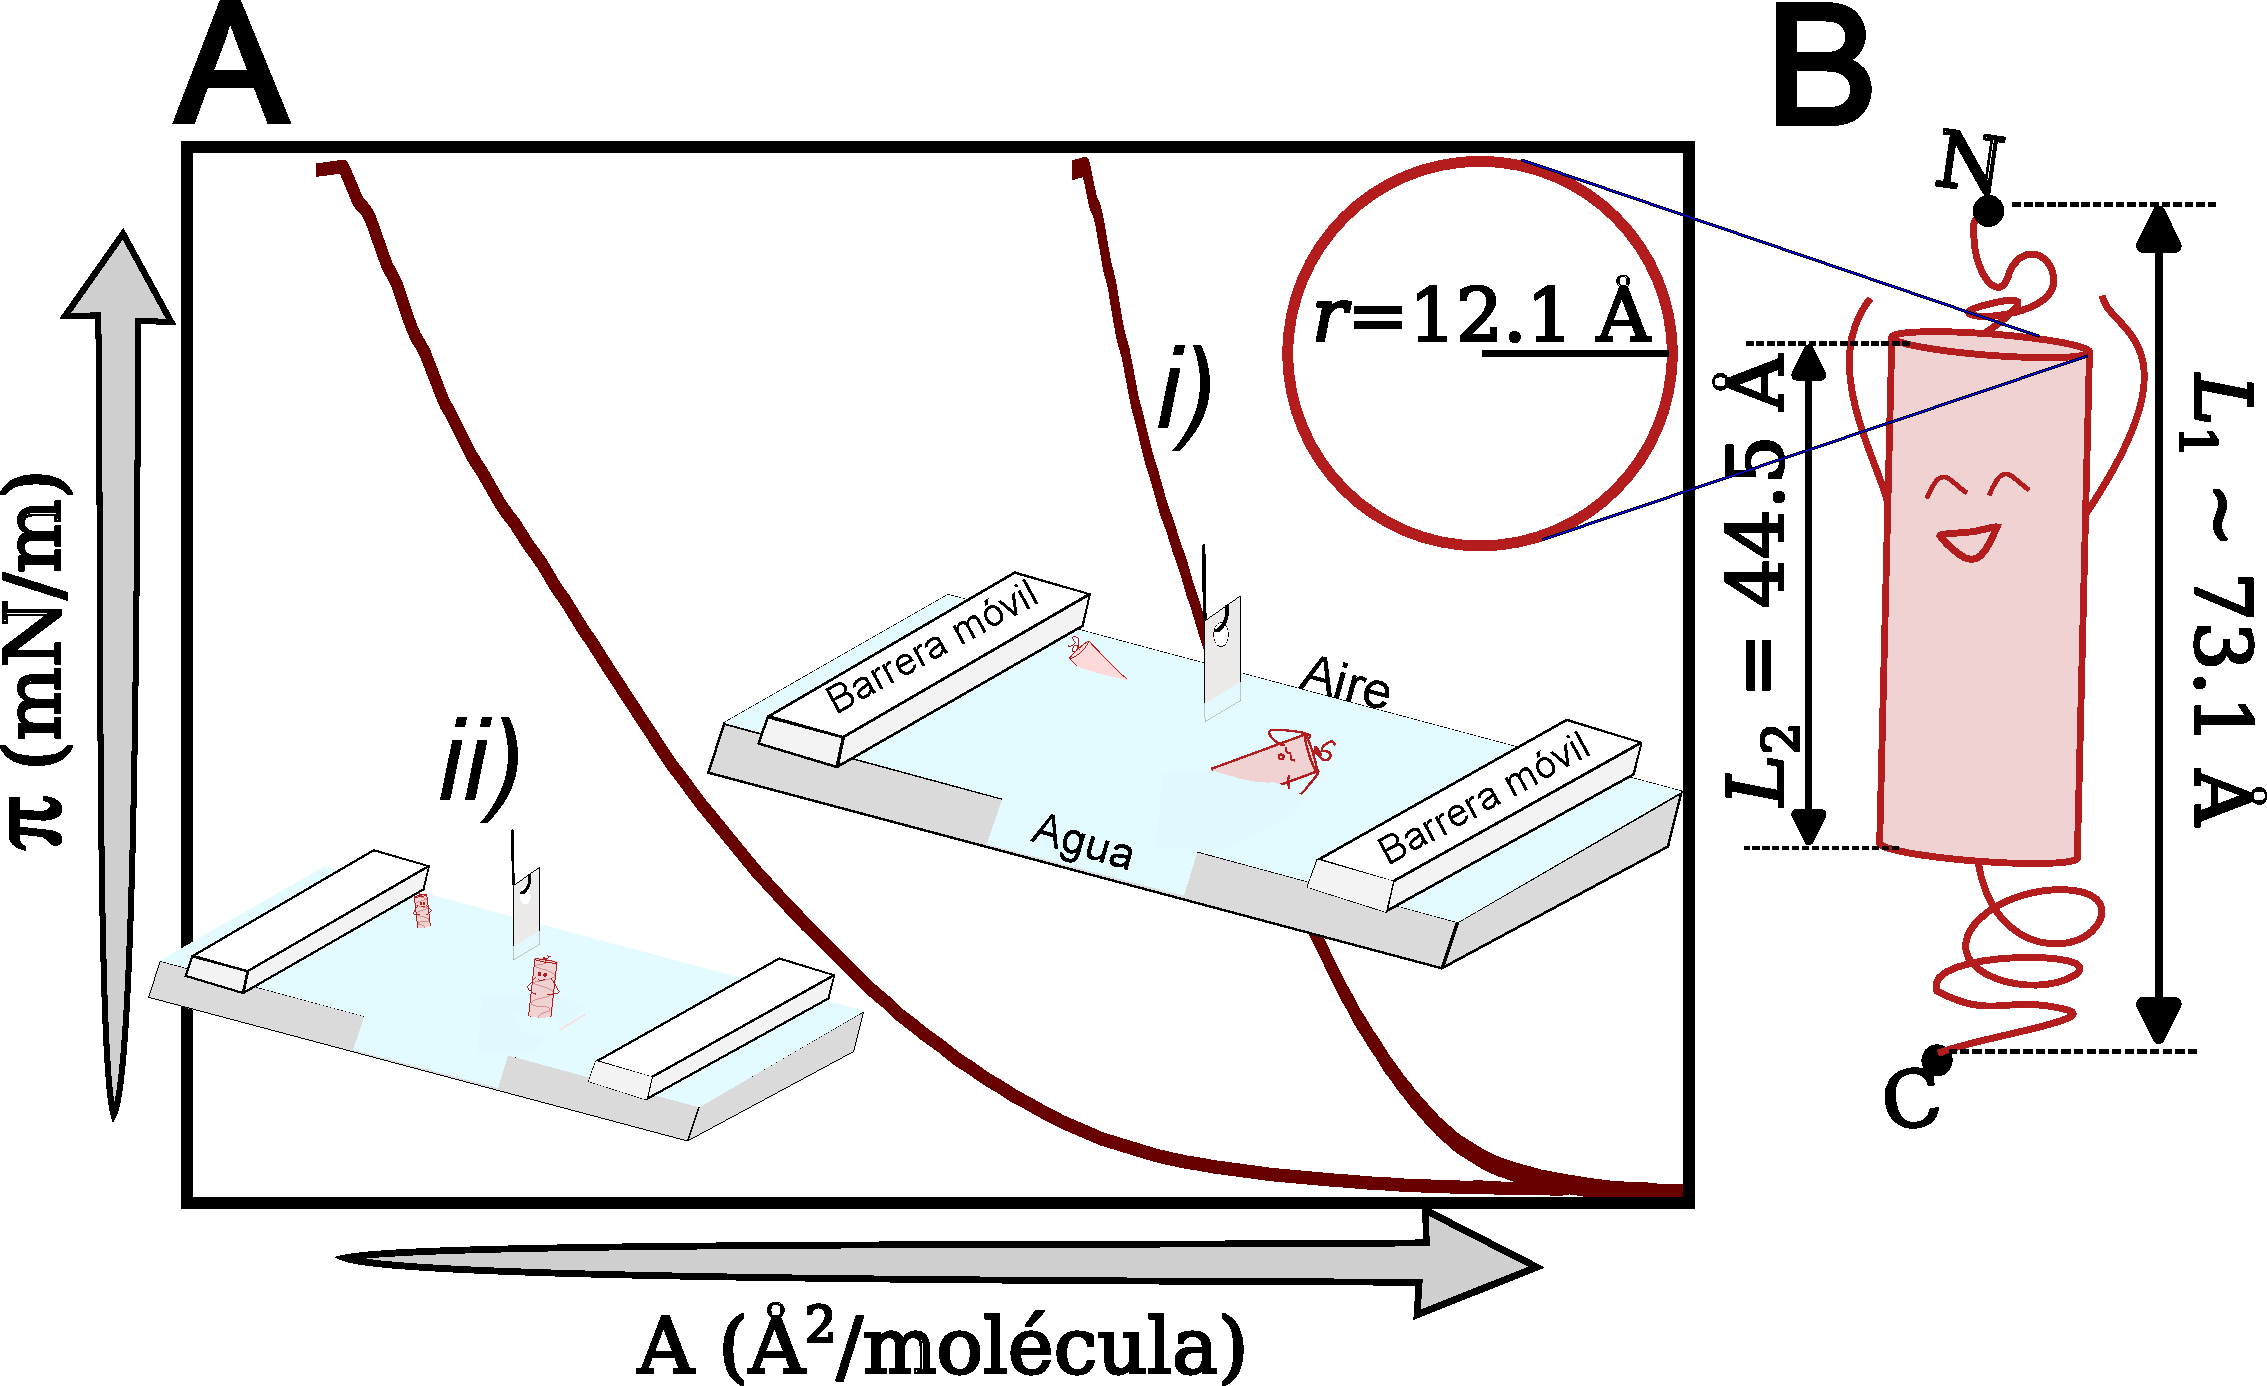
\includegraphics[width=0.85\linewidth]{fig/01_expe/orienta_pept2.pdf}
	\caption[Modelo de posible orientación de $\alpha$-hélice en el plano de una monocapa.]{Modelo de posible orientación de hélice $\alpha$ en el plano de una monocapa.}
        \index{orientacion}
    \label{fig:orientTM}
\end{figure}
%%%%%%%%%%%%%%%%%%%%% Fin %%%%%%%%%%%%%%%%%%%%%%%%


Ambos péptidos presentan actividad superficial en monocapas de Langmuir (\textbf{figura}~\ref{fig:area_pi_pept}A). Forman monocapas estables que pueden ser comprimidas en al menos dos ciclos de compresión-descompresión sin perder material por partición a la subfase. La siembra de 0.5 nmoles no produjo un aumento de presión significativamente diferente de cero y corresponde a un área de $\Xapprox 2500$ Å\textsuperscript{2}/molécula. A 5 mN/m, los péptidos se han compactado y el área molecular es de  $\Xapprox 1300$ Å\textsuperscript{2}. A presiones de  35 y 42 mN/m para $\alpha$IIb y $\beta$3, el área molecular fue de $\Xapprox 482$ \textpm 52 y $\Xapprox 593$ \textpm 20 Å\textsuperscript{2} para $\alpha$IIb y $\beta$3 respectivamente. Estos valores de área molecular indican que los péptidos tiene un radio de 12.4 Å para $\alpha$IIb y 13.7 Å para $\beta$3, y tienden a organizarse perpendicularmente al plano de la monocapa en estructura hélice $\alpha$ tal como se sugirió en la \textbf{figura} ~\ref{fig:orientTM}A-\textit{ii}. Algunos autores \cite{Barlow1988, Kato2015,Ionov2000,Weder2003} han reportado un radio promedio de 5.0 Å en hélices $\alpha$ el cual da un área de  78.5 Å\textsuperscript{2} y más reciente Mura et al. \cite{Mura2013} reportó un radio de 10 Å valor que correspondería un área molecular de 314.6 Å\textsuperscript{2}. Las áreas para los dos péptidos se encuentran cercanos a éste último valor. Por último nos preguntamos, cuál es la orientación de los péptidos, es decir, ¿\textit{del N- al C-terminal ó del C- al N-terminal}?. El no colapso de la monocapa estaría dado por las posibles fluctuaciones de la región que no tiene estructura secundaria definida (segmento \ac{ic}), por tanto a presiones bajas estas regiones son las que se localizan preferentemente en la subfase mientras que las  hélice $\alpha$, región hidrofóbica, se orienta hacia el aire. A medida que se comprime la monocapa, las colas forman ``loops'' que aumentan de tamaño y pueden oscilar a medida que se compacta y por lo tanto no se llega a una presión de colapso (ver \textbf{figura} \ref{fig:mono_pept}, flechas \textcolor{blue}{\faLongArrowRight}), algo similar reportaron Toimil et al. \cite{Toimil2012} para álbumina sérica humana. A un presión 35 mN/m el péptido $\alpha$IIb presentó un áréa molecular ligeramente mayor al esperado teóricamente (460 Å\textsuperscript{2}), éste valor se calculó teniendo en cuenta sólo la región con estrucutura secundaria hélice $\alpha$, de igual forma con $\beta$3. El área experimental de $\beta$3 es más grande comparado con $\alpha$IIb, y puede ser porque $\beta$3 tiene un dominio citoplasmático más largo no estructurado. \\

%%%%%%%%%%%%%%%%%%%%%Fig. Isotermas de compresión peptidos %%%%%%%%%%%%%%%%%%%%%

\begin{figure}[h!] % supposedly places it here ...
    \centering
	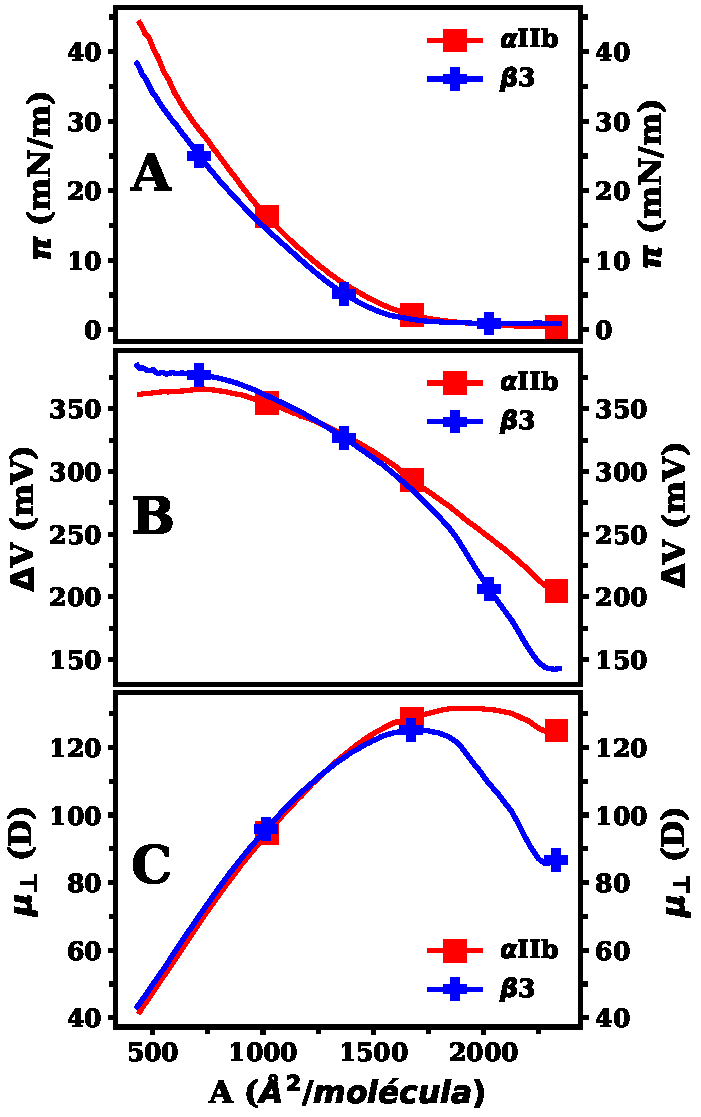
\includegraphics[width=0.5\linewidth]{fig/01_expe/mono/area_pi_peptidos.pdf}
	\caption[Isotermas de compresión en la interfase agua/aire para péptidos puros.]{Isotermas de compresión en la interfase agua/aire para péptidos puros. \textbf{A)} Presión superficial ($\pi$), \textbf{B)} potencial de superficie $\Delta V$ y  \textbf{C)} momento dipolar total, respecto al área molecular media (\textbf{A)}}.
        \index{area_pi_pept}
    \label{fig:area_pi_pept}
\end{figure}
%%%%%%%%%%%%%%%%%%%%% Fin %%%%%%%%%%%%%%%%%%%%%%%%

Helmholtz propone que en una monocapa las especies químicas que estan cerca de la superficie del agua presentan una orientación específica \hl{REF}. Ésta orientación viene dada por los dipolos de cada especie y puede describirse por la siguiente ecuación,

\begin{equation}
    \label{ecu:potencial}
    \Delta V =  \frac{12 \Pi \mu_\perp}{A}
\end{equation}

Donde $\Delta V$ es el potencial de superficie (mV) medido entre el seno de la solución acuosa y la \hl{fase gaseosa (aire)}, \textit{A} el área molecular (Å\textsuperscript{2}), $\Pi$ es constante  y $\mu_\perp$ el momento dipolar total de superficie ($\mu_\perp$). El $\Delta V$, medido en una monocapa tiene tres contribuciones: 1) los dipolos ordenados de las moléculas adsorbidas, 2) los dipolos de las moléculas de agua ordenadas en la zona de la superficie, 3) el dipolo generado por la doble capa iónica de Gouy-Chapman  en en caso que las moléculas adsorbidas tengnan cargas netas \cite{Brockman1994,Electronics1994}. Se observó que aún cuando la presión de superficie es indistinguible de cero, el $\Delta V$ es significativamente grande y alcanza valores de entre 200 y 150 mV para $\alpha$IIb y $\beta$3 respectivamente (\textbf{figura} \ref{fig:area_pi_pept}B). 
%%%$\mu_\perp$ = $\mu_1$ + $\mu_2$ + $\mu_3$, $\mu_1$ es la contribución de las moléculas de agua orientadas al rededor de las caras hidrofílicas de la proteína, $\mu_2$ y $\mu_3$ contribuciones hidrofílica e hidrofóbica de la proteína que esta en contacto con la superficie 
En los dos péptidos el $\mu_\perp$ inicia con valores relativamente altos (\textbf{figura} ~\ref{fig:area_pi_pept}C) y a medida que se comprime lateralmente va dismuniyendo hasta alcanzar los $\Xapprox 43$ D al valor mínimo área molecular, esta tendencia abre la posibilidad a realizar el siguiente planteamiento de reorganización, inicialmente los péptidos se encuentran con una supercie de contacto mayor expuesta al agua y por lo tanto, hay alta densidad de carga que contribuye al $\mu_\perp$  (\textbf{figura} \ref{fig:mono_pept}A-B-C, sin embargo al compactarse lateralmente, los péptidos tienen a orientarse verticalmente, exponiendo menos residuos al superficie de la monocapa, disminuyendo la densidad de cargar, finalmente se llega a un estado donde estan lo sufientemente  compactactados que todo lo que tiene estructura $\alpha$ hélice queda expuesto al aire y la única parte que contribuye al $\Delta$V y/o $\mu_\perp$ es la región que fluctúa de estrucutra y que tiene mayor caracter polar; un planteamiento similar realizó Maget \cite{Maget-Dana1999}.

%%%% \textbf{figura} modelo compactacion pept en monocapas%%%
\begin{figure}[H] 
    \centering
	
\includegraphics[width=0.99\linewidth]{fig/01_expe/mono_pept.pdf}
	\caption{Modelo de reorganización de los péptidos en monocapas de Langmuir y fluctuación de estrucuta secundaria en segmento intracelular para los péptidos $\alpha$IIb y  $\beta$3.}
        \index{mono_pept}
    \label{fig:mono_pept}
\end{figure}
%%%%%%%%%%%%%%%%%%%%% Fin %%%%%%%%%%%%%%%%%%%%%%%%} 

Para tener una mejor idea de lo planteado anteriormente acerca de cómo se orientan los péptidos la monocapa de Langmuir, se realizó un análisis de la hidrofobicidad promedio por residuo <H> \, y del momento hidrofóbico $\mu_H$ para cada péptido (ver \textbf{tabla} ~\ref{tab:mu_hidrofo}). En los dos péptidos, el domino \ac{tm} presenta mayor <H> \,  respecto a los dominios \ac{ec} e \ac{ic}, principalmente dado por la cantidad de residuos hidrofóbicos (\textbf{figura} ~\ref{fig:mu_hidrofo}, resaltados en amarillo \begin{tikzpicture}
  \node[draw, circle, fill=yellow, line width=0.5pt, inner sep=1pt, scale=0.6, font=\color{yellow}] {\faCircle}; \end{tikzpicture}). El <H> \, del dominio \ac{ec} es más grande (0.693\textgreater\!\textgreater -0.091) que dominio \ac{ic} del péptido $\alpha$IIb, además, el domino \ac{ic} presenta cuatro cargas negativas comparadas a una carga positiva del dominio \ac{ec}. El péptido $\beta$3 tiene 25 residuos más que $\alpha$IIb en el dominio \ac{ic} (\textbf{figura} ~\ref{fig:mu_hidrofo}, ``\textbf{55-79}''), éstos últimos residuos que a aportan un caracter hidrofóbico aunque sigue siendo menor comparado al dominio \ac{ec} (0.163\textless\!\textless 0.360), además, también hay la presencia de una carga positiva. Por tanto en los dos péptidos, es más probable que el dominio \ac{ic} interactúe con la fase acuosa, lo cual conduce a plantear que los péptidos se orientan del \textit{del N- al C-terminal}.


%%%%Tabla resumen de H_mu%%%%
\begin{table}[H]
%\begin{wraptable}{r}{0.50\textwidth}
%\vspace{-0.7cm} 
\centering
\begin{threeparttable}
\centering
\caption{Resumen hidrofobicidad y carga para los dominios \ac{ec}, \ac{tm} y \ac{ic} de péptidos $\alpha$IIb y  $\beta$3.}\label{tab:mu_hidrofo}
\begin{tabular}{@{}llccl@{}}
\toprule
Péptido     & N° Residuo             & <H>      	& <$\mu_H$> 	& z  \\ \midrule
$\alpha$IIb & \multirow{2}{*}{1-11 \; (EC) }  & 0.185  	& 0.273 		& 1- \\
$\beta$3    &                        & 0.360  	& 0.341 		& 0  \vspace{3mm} \\
$\alpha$IIb & \multirow{2}{*}{12-36 \;(TM)} & 1.182  	& 0.133 		& 1+ \\
$\beta$3    &                        & 1.183  	& 0.121 		& 1+ \vspace{3mm} \\
$\alpha$IIb & \multirow{2}{*}{37-54 \;(IC)} & -0.091 	& 0.263 		& 4- \\
$\beta$3    &                        & -0.091 	& 0.184 		& 0  \vspace{3mm} \\
$\beta$3    & 55-79 \;(IC)                  & 0.163  	& 0.233 		& 1+ \\ \bottomrule
\scriptsize{\ac{ec}: \acl{ec}} & \scriptsize{\ac{tm}: \acl{tm}} & \scriptsize{\ac{ic}: \acl{ic}}
\end{tabular}
\end{threeparttable}
%\vspace{-0.5cm} 
%\end{wraptable}
\end{table}
%%%%%Fin tabla%%%%%



\hl{Es importante destacar que la evaluación de la actividad superficial comprende la integración de múltiples factores contribuyentes, entre ellos la anfipaticidad, el tamaño molecular, la flexibilidad estructural, la carga neta y las interacciones intramoleculares. Esta complejidad inherente en la composición y el comportamiento de las moléculas subraya las dificultades inherentes en la medición precisa del potencial de superficie. Además, es relevante reconocer que, dadas estas variadas influencias, los resultados experimentales relativos a esta propiedad suelen exhibir una considerable variabilidad, manifestándose en una dispersión significativa en comparación con los valores teóricos anticipados. Esta observación resalta la necesidad de un enfoque meticuloso y detallado en la interpretación de los datos experimentales, considerando la gama de variables que pueden afectar las mediciones del potencial de superficie..}\\

\begin{figure}[H] % supposedly places it here ...
    \centering
	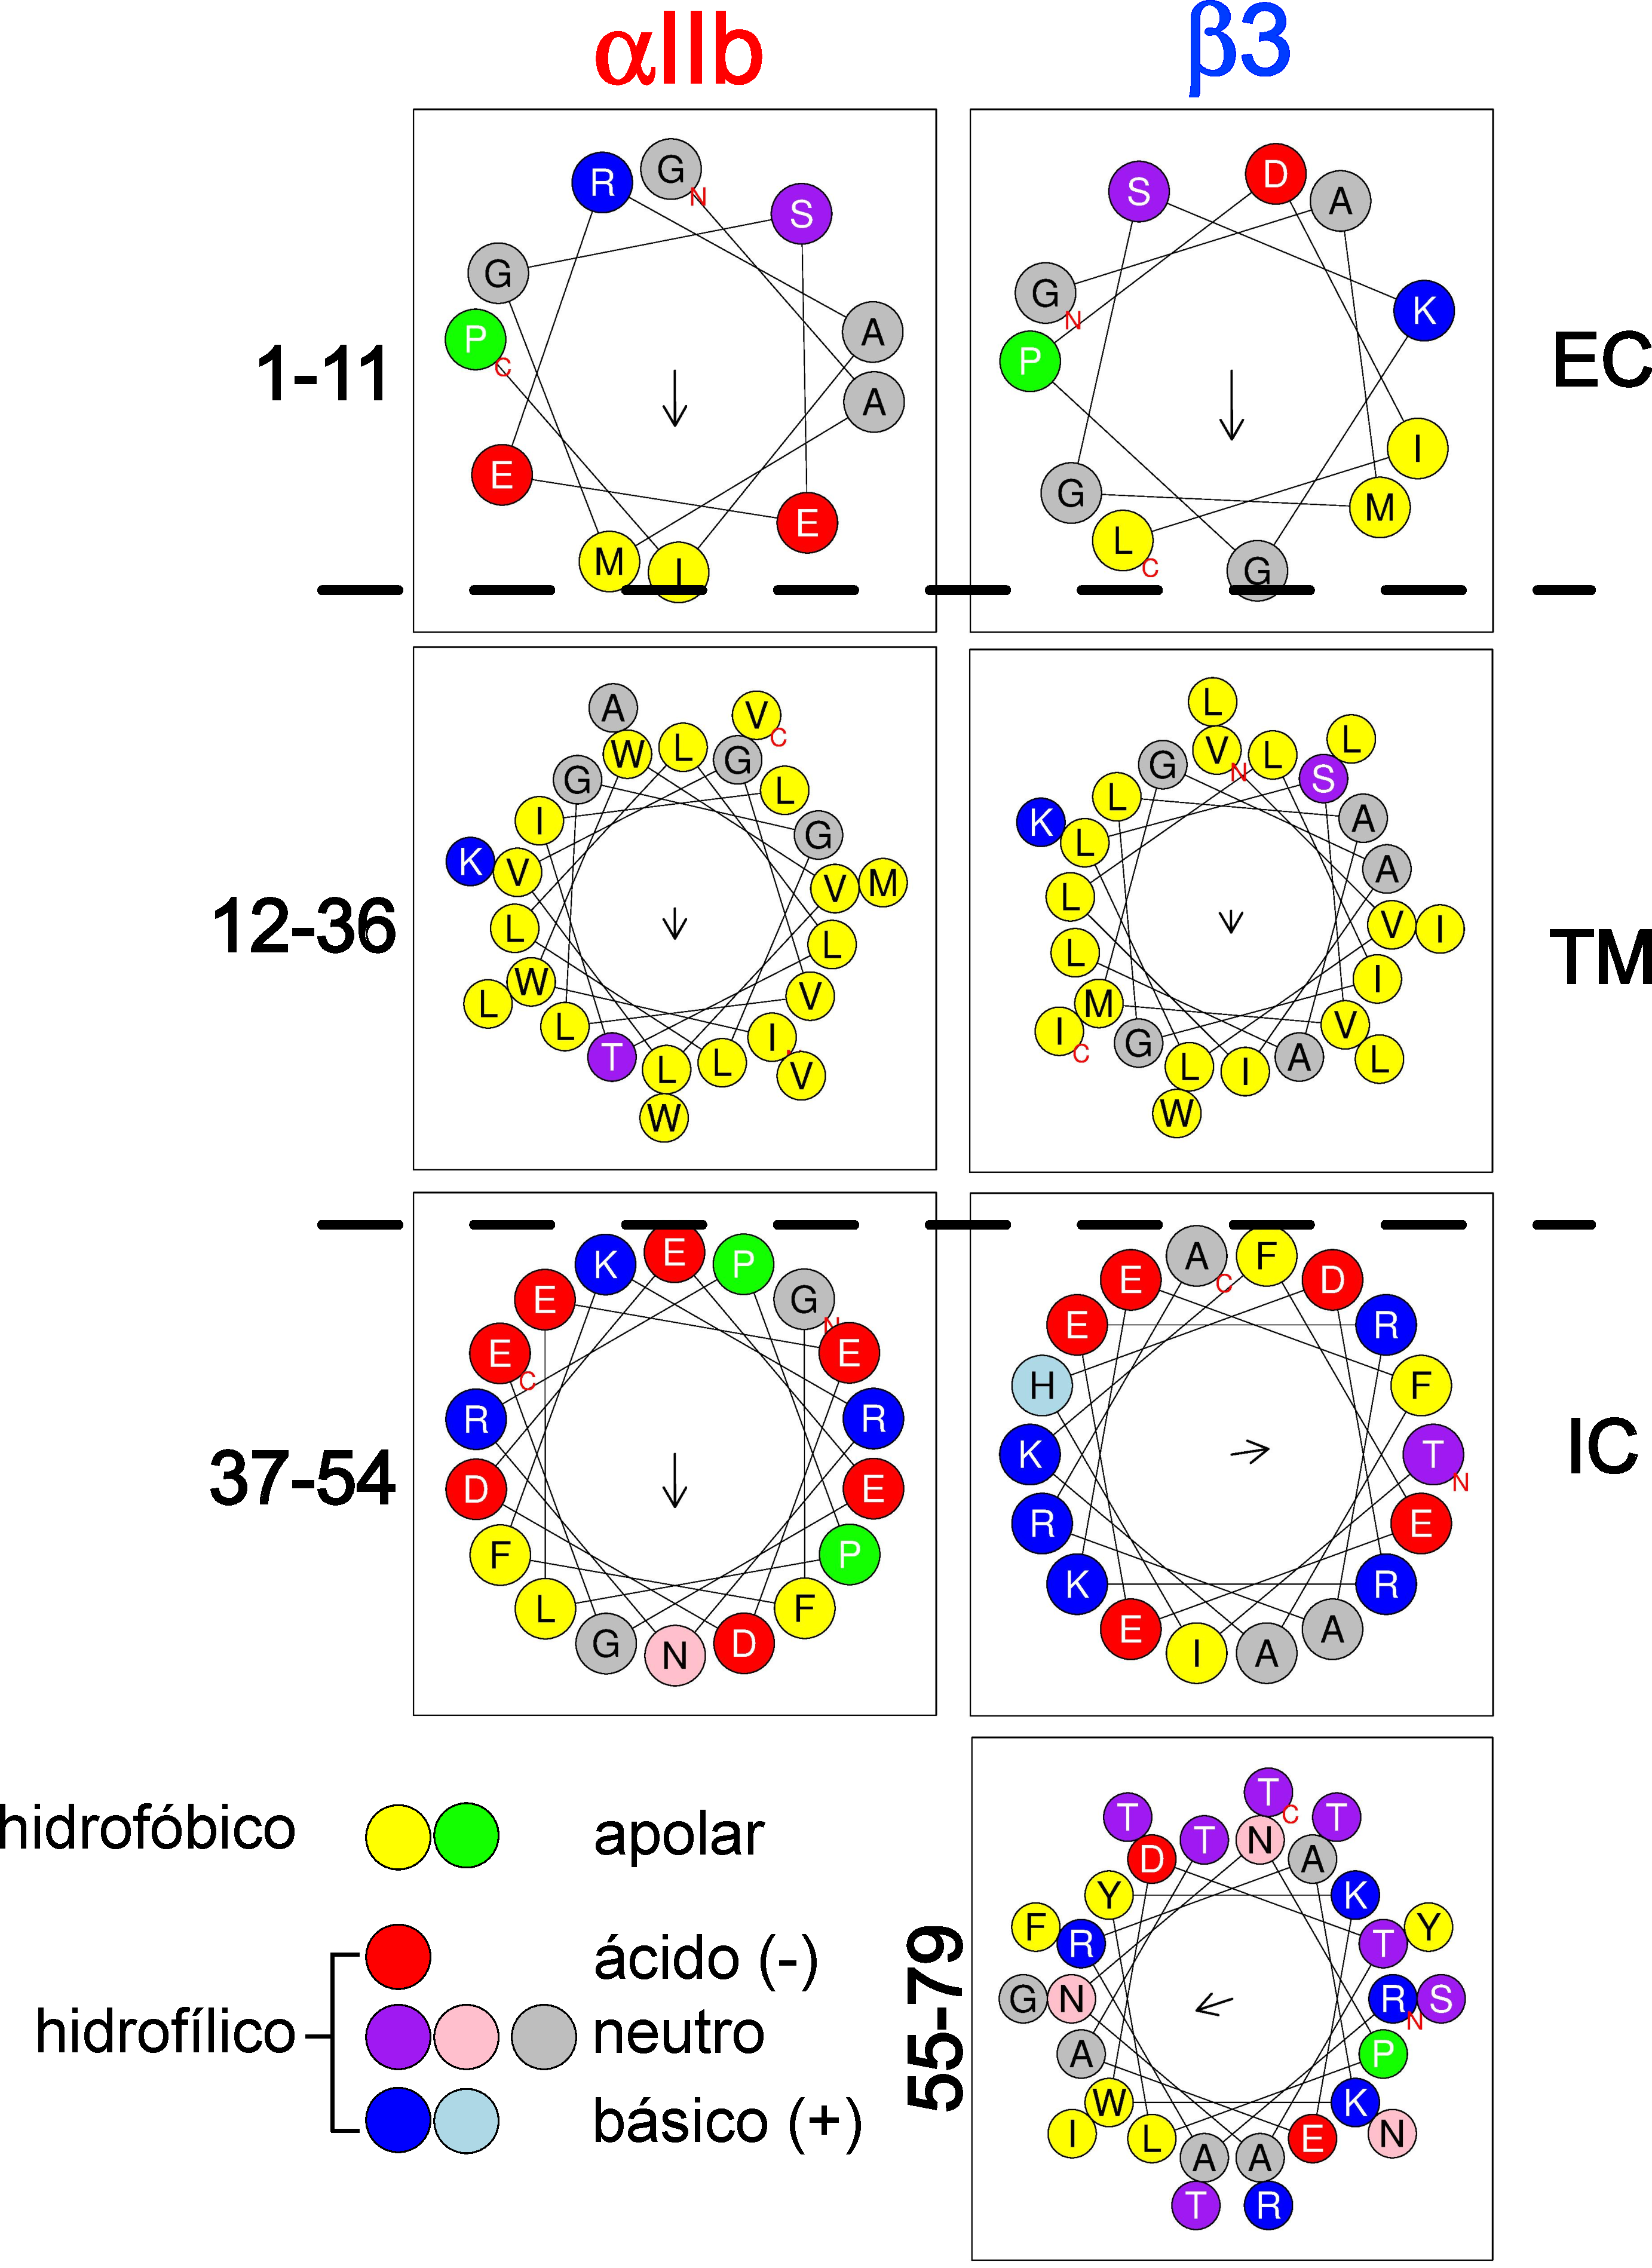
\includegraphics[width=0.7\linewidth]{fig/01_expe/secuencias_alfa_beta.pdf}
	\caption[Proyección circular de la hélice para las secuencias de los segmentos transmembrana $\alpha$IIb y  $\beta$3.]{Proyección circular de la hélice para las secuencias de los segmentos transmembrana $\alpha$IIb y  $\beta$3. La fecha (\textrightarrow) en el centro indica la magnitud y la dirección del momento hidrofóbico <$\mu_H$>. La proyección se realizó con el software HeliQuest  (\url{https://heliquest.ipmc.cnrs.fr}).}
        \index{mu_hidrofo}
    \label{fig:mu_hidrofo}
\end{figure}
%%%%%%%%%%%%%%%%%%%%% Fin %%%%%%%%%%%%%%%%%%%%%%%%

\section{Monocapas de Langmuir para mezclas lípido-péptido}\label{sect:mono_mezclas}

Se realizaron isotermas de compresión de lípido puro (\ac{popc}, PCPG, \ac{dppc}) y mezclas lípido-péptido ($\alpha$IIb ó $\beta$3) en concentraciones de crecientes de péptido desde 0.0 a 7.0\% mol. En la \textbf{figura} ~\ref{fig:area_pi_all}, panel superior de  se muestran las mezclas de lípido-$\alpha$II y en el inferior las mezclas lípido-$\beta$3. En todos los experimentos se realizaron 3 ciclos de compresión-expansión para evaluar la estabilidad del film lípido-péptido. Para la mezcla \ac{popc}/$\alpha$IIb se observó que en todos los casos se produjo un corrimiento a áreas mayores respecto al lípído puro y este pareciera ser mayor con el incremento de la concentración de péptido. En PCPG/$\alpha$IIb se observó que hay el lípido tiene a compactarse o por lo menos a estar más cerca de la isoterma de la mezcla pura PCPG; y para la mezcla \ac{dppc}/$\alpha$IIb el efecto de expansión fue más notorio en los tres sistemas estudiados, incluso en todas la concentraciones se observó que la pretransición en \ac{dppc} no se percibe ya con 2.0\% de péptido (\textcolor{emerald}{\rotatebox{0}{\faStar}}). Respecto a las mezclas en presencia de $\beta$3, presentaron compartamientos similares a lo observado con el péptido $\alpha$IIb, en la mezcla con PCPG el corrimiento a areas menores es más marcado en concentraciones de 2.0\% y 3.5\% (\textcolor{falured}{\rotatebox{90}{\faPlay}}).
Comparando un poco más en detalle el efecto de los dos péptidos,  en las monocapas de \ac{popc}, a 5.0\% (\textcolor{goldenpoppy}{\faCircle}) de $\alpha$IIb se desplaza a áreas menores comparado las concentraciones más bajas que iba aumentando pero luego a 7.0\% (\textcolor{deepmagenta}{$\pentagonblack$}) se recupera dicha tendencia, mientras que en presencia de $\beta$3 sucede el mismo efecto pero a 2.0\% y luego se produce el corrimiento a áreas mayores. Para la mezlca binaria de lípidos PCPG, pareciera que a bajas concentraciones de péptido 2.0\% y 3.5\% se produce en efecto de compactación, siendo más notorio cuando se trata de $\beta$3. En presencia de \ac{dppc} el corrimiento hacia áreas mayores al incrementar la concentración de péptido se cumple para ambos péptidos, sin embargo, en presencia de $\beta$3 esa tendencia se sigue hasta 5.0\% porque luego a 7.0\% baja a corrimientos similares al 2.0\% de $\beta$3.

%%%%%%%%%%%%%%%%%%%%%Fig. Isotermas de compresión %%%%%%%%%%%%%%%%%%%%%
\begin{figure}[H] % supposedly places it here ...
    \centering
	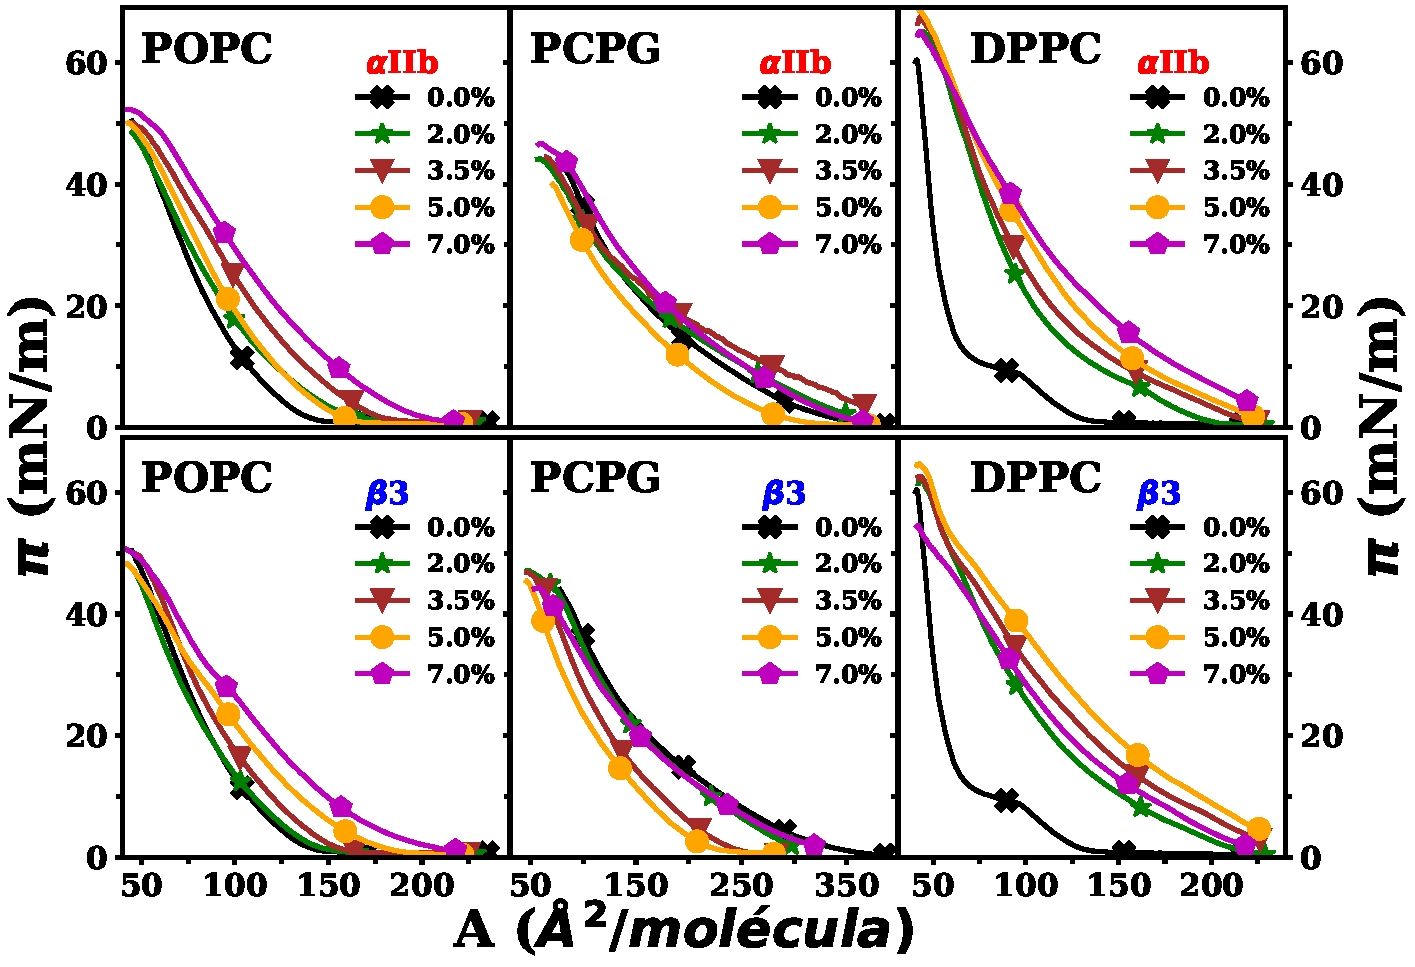
\includegraphics[width=0.99\linewidth]{fig/01_expe/mono/area_pi_all.pdf}
\caption[Isotermas de compresión, presión superficial -- área molecular promedio (\boldmath{$\pi$}--A) en la interfase aire-agua.]{Isotermas de compresión, presión superficial -- área molecular promedio (\boldmath{$\pi$}--A) en la interfase aire-agua de los sistemas lípido-péptido (lípidos = POPC, POPC:POPG  70:30 llamdao PCPG y  DPPC). Panel superir lípdio/$\alpha$IIb, panel inferior lípido/$\beta$3; las concentraciones crecientes de péptido están idicadas en cada sub\textbf{figura} por marcadores respectivos.}
        \index{area_pi_all}
    \label{fig:area_pi_all}
\end{figure}
%%%%%%%%%%%%%%%%%%%%% Fin %%%%%%%%%%%%%%%%%%%%%%%%

%Dado que de los gráficos anteriores no se puede realizar conclusiones generales de cómo interactúan los péptidos con los lípidos, se procedió a realizar un análisis del área molecular promedio vs el porcentaje de péptido a diferentes presiones con la finalidad de encontrar alguna tendencia más evidente para cada sistema estudiado (ver la siguiete sección  ~\ref{AvsMol}).


%%%%%%%%%% Àrea Vs %mol
\section{Análisis de la miscibilidad  de mezclas lípido-péptido}{\label{AvsMol}}

Como previamente se observó las monocapas monomoleculares permiten evaluar las característi de empaquetamiento molecular, además también es posible obtener una idea de cómo es el grado de miscibilidad lípido-péptido comparando el área molecular promedio de la mezcla a una dada presión superficial (propiedad aditiva). El área de una mezcla es comparada con las área media moleculares de cada componente por separado a una dada presión superficial. Las áreas de las mezclas ideales $A_{ideal}$ para dos componentes fue calculada según la ecuación ~\ref{ecua:Aideal} \citep{Ali1994} a las presiones de 2 y 30 mN/m,

\begin{equation}
    \label{ecua:Aideal}
    A_{ideal} = \left[X_{\text{L}}A_{\text{L}} + X_{\text{P}}A_{\text{P}}\right]_\pi
\end{equation}

Donde $A_{L,P}$ son las áreas moleculares promedio y $X_{L,P}$ son las fracciones molares del lípido y péptido respectivamente a una determinada presión. Los componentes de la mezcla tendrán un área $A_{ideal}$ si estos no interaccionan, o lo hacen hacen idealmente, por lo tanto cualquier desviación de la idealidad es atribuída a interacciones específicas que pueden ser atractivas (el área observada es menor al $A_{ideal}$) o repulsivas (el área observada es mayores al $A_{ideal}$) entre los componentes. 
A partir de los datos de la \textbf{figura} ~\ref{fig:area_pi_all} se calcularon las áreas $A_{ideal}$  para cada mezcla a las presiones mencionadas y se compararon  respecto a los datos experimentales.
A una presión superficial de 2 mN/m (\textbf{figura} ~\ref{fig:Fig_AreaVsMoles}--panel superior), las áreas moleculares promedio observadas sugieren que ambos péptidos presentan interacciones atractivas lípido-péptido en los sistemas \ac{popc} y PCPG, mientras que en la mezcla \ac{dppc}-péptido el comportamiento es de caracter repulsivo a concentraciones de 2.0\% a 5.0\%.
En el panel inferior (\textbf{figura} ~\ref{fig:Fig_AreaVsMoles}) se muestra el mismo análisis a 30 mN/m y la tendencia de los datos experimentales es similar a los observado a 2 mN/m en para todas las mezclas lípido-péptido. 

%%%Tabla con carácterísticas de los lípidos
\begin{table}[H]
\centering
\begin{threeparttable}
\centering
\caption[Generalidades lípidos]{Generalidades lípidos}\label{tab:lipidos}
%\begin{wraptable}{r}{0.52\textwidth}
%\vspace{-0.8cm} %%%Posiciona a una altura en la hoja
\begin{tabular}{lccc}
\hline
Lípido                       & \cellcolor[HTML]{EFEFEF}Enlace & \cellcolor[HTML]{EFEFEF}Fase a 25°C & \cellcolor[HTML]{EFEFEF}Carga neta \\ \hline
\cellcolor[HTML]{CBCEFB}POPC & 16:0-18:1                      & LE                                  & 0   \\
\cellcolor[HTML]{CBCEFB}POPG & 16:0-18:1                      & LE                                  & 1-- \\
\cellcolor[HTML]{CBCEFB}DPPC & 16:0                           & múltiples                           & 0 \\
\hline\\
\end{tabular}
%    \vspace{-1.51cm} %%%espacio entre texto y botton table
%%    \end{wraptable} 
\end{threeparttable}
\end{table}
%%%%%Fin tabla%%%%%


%%%%%%%%%%%%%%%%%%%%%% Fig A Vs %mol %%%%%%%%%%%%%%%%%%%%%%%%
\begin{figure}[h] % supposedly places it here ...
    \centering
	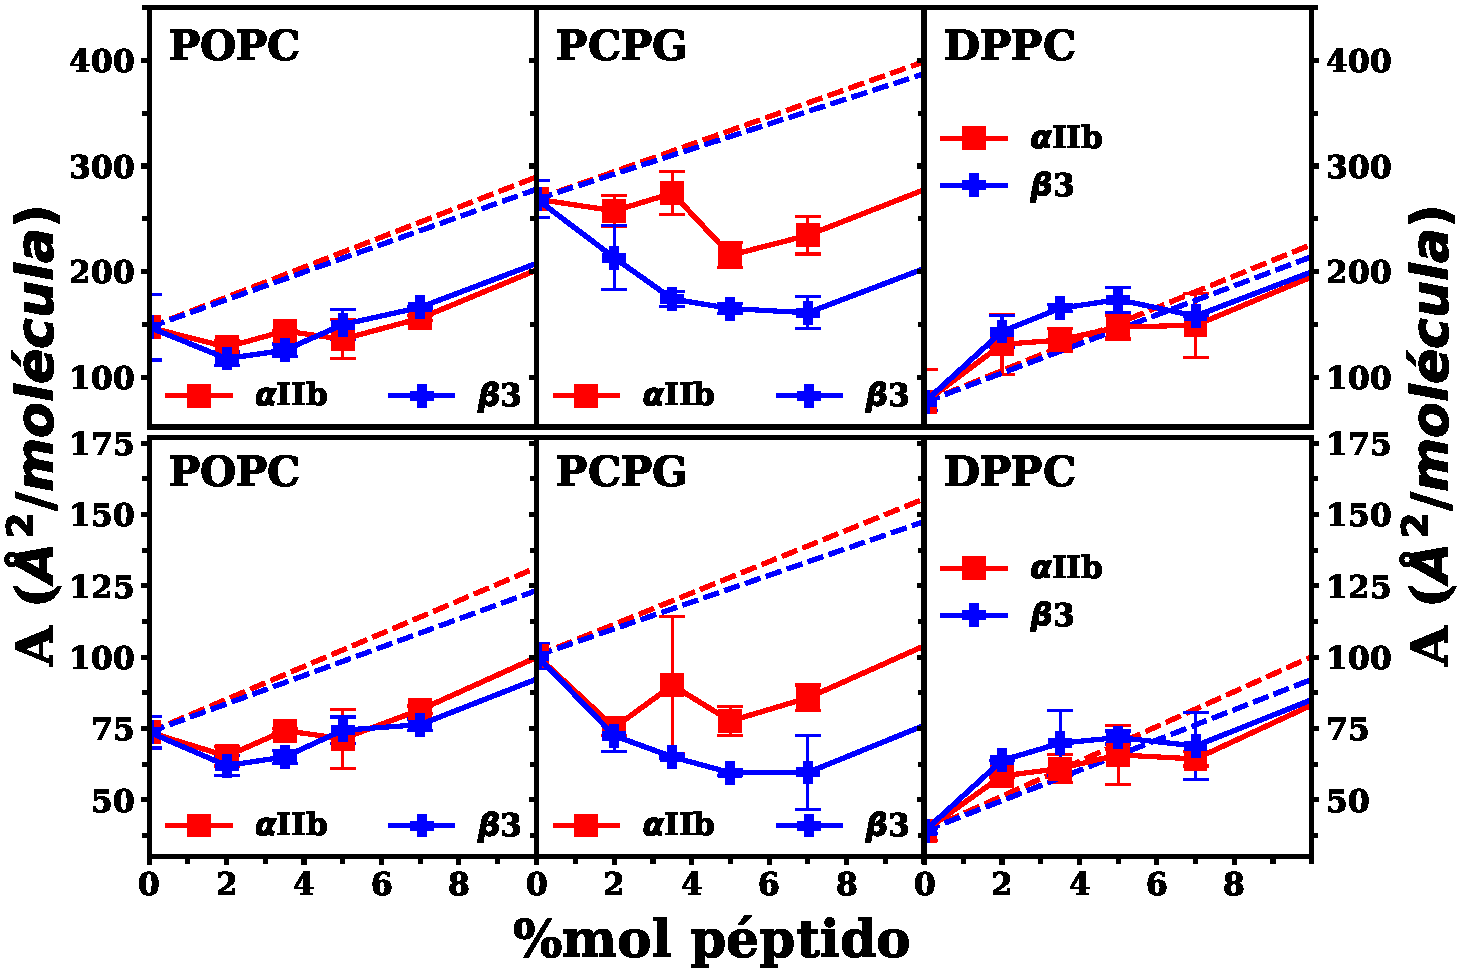
\includegraphics[width=0.99\linewidth]{fig/01_expe/mono/Aideales_all2.pdf}
	\caption[Área molecular promedio Vs porcentaje molar (A--\%mol péptido) para cada sistema lípido-péptido.]{Área molecular promedio Vs porcentaje molar (A--\%mol péptido) para cada sistema lípido-péptido (lípidos = POPC, POPC:POPG  70:30 llamdao PCPG y  DPPC). Panel superior e inferior 2 y 30 mN/m, respectivamente. Las líneas  - - - indican la curva de idealidad para las mezclas.}

     \index{Fig_AreaVsMoles}
    \label{fig:Fig_AreaVsMoles}
\end{figure}
%%%%%%%%%%%%%%%%%%%%% Fin %%%%%%%%%%%%%%%%%%%%%%%%


Para comprender un poco más en detalle lo que podría estar sucediendo a nivel molecular, veamos algunas características de los lípidos en particular. En la \textbf{tabla} \ref{tab:lipidos} vemos que el \ac{popc} y POPG tiene el mismo tipo de enlaces en la cadena hidrofóbica y también el mismo largo de cadena (átomos de carbono) y misma fase a temperatura ambiente (líquido expandido, LE),  con la diferencia el POPG tiene carga neta negatiga mientras que el \ac{popc} es zwiteriónico, por otra parte el \ac{dppc} es un lípido saturado (no posee dobles enlaces), es de 16 carbonos en ambas cadenas hidrofóficas y tiene múltiples transiciones de fase. Con base en estas características, retomando lo observado en la \textbf{figura} ~\ref{fig:Fig_AreaVsMoles} vemos que ambos péptidos tienden a compactar los lípidos con LE e interaccionan de forma repulsiva (expanden) el \ac{dppc} que presenta pricipalmente una fase líquido condensado (LC). También se vio que en la mezcla PCPG que tiene carga negativa, interacciona preferentemente con el péptido $\beta$3 que tiene carga neta de 2+, comparado con el $\alpha$IIb.



%%%%Paper Properties of the Langmuir and Langmuir–Blodgett monolayers
%%%%of cholesterol‑cyclosporine A on water and polymer support
%%%%https://doi.org/10.1007/s10450-019-00117-2

Recientemente los autores Socas, L. y Ambroggio, E. \cite{Socas2018,Socas2023} propusieron un modelo matemático para comparar isotermas de compresión en monocapas. En lugar de comparar las isotermas a presiones definidas, como se realizó anteriormente a 2 y 30 mN/m, el modelo compara cuantitativamente las isotermas en todo el rango de presiones. La comparativa de dos isotermas distintas, designadas respectivamente como la isoterma de interés e isoterma de referencia, implica la instauración de un parámetro denominado factor $\Lambda$ definido por dos parámetros: 

\begin{equation}
    \label{ecua:lambda}
    \Lambda = \left(\lambda,r^2 \right)
\end{equation}

Donde $\lambda$ representa un factor de \textit{distancia} entre las áreas moleculares media de las isotermas y r$^2$ el grado de “similitud” entre la forma de las curvas a lo largo de todo el rango de presiones comunes en ambas isotermas. Primero se determina el rango de valores de presión que son comunes a ambas isotermas  (de referencia y de interés) y se emplea un algoritmo de regresión no lineal para encontrar el  valor de λ que minimice la diferencia de cuadrados entre los valores del área molecular promedio (\textbf{A}) de la isoterma de interés y los calculados para cada valor de presión según:

\begin{equation}
    \label{ecua:lambda2}
    \textbf{A}\text{(} \pi \text{)} = \lambda \; \text{x} \; \textbf{A}_{\text{referencia}} \text{(} \pi \text{)}
\end{equation}

 Finalmente se procede a calcular el coeficiente de determinación (r$^2$), que proporciona una medida cuantitativa de la congruencia entre la curva isoterma resultante y la curva isoterma de interés. Los valores obtenidos para  r$^2$ y $\lambda$ se abordan de la siguiente manera:

%%%%%Tabla de significado lambda%%%%%%%%%%%%
\begin{table}[H]
%\centering
\begin{threeparttable}
\centering
%\caption[Factor $\Lambda$ para comparar cuantitativamente isotermas]{Factor $\Lambda$ para comparar cuantitativamente isotermas}\label{tab:lambda}
\begin{tabular}{lcl}
\rowcolor[HTML]{ECF4FF} 
\multicolumn{1}{r}{\cellcolor[HTML]{ECF4FF}r$^2$ y $\lambda$ = 1} &  & Isotermas idénticas                \\
\rowcolor[HTML]{CBCEFB} 
\cellcolor[HTML]{CBCEFB}                            & $\lambda$ \textgreater{} 1 & Similar en forma con desplazamiento hacia áreas moleculares \textbf{mayores} \\
\rowcolor[HTML]{CBCEFB} 
\multirow{-2}{*}{\cellcolor[HTML]{CBCEFB}r$^2$ $\Xapprox 1$ } & $\lambda$ \textless{} 1 & Similar en forma con desplazamiento hacia áreas moleculares \textbf{menores} \\
\rowcolor[HTML]{ECF4FF} 
r$^2$ \textless{}\textless{} 1                                                           &  & Las isotermas no se parecen en forma
\end{tabular}
\end{threeparttable}
\end{table}
%%%%%Fin tabla%%%%%


%%%%%%%%%%%%%%%%%%%%%% Tabla LAMBDA %%%%%%%%%%%%%%%%%%%%%%%%

\begin{figure}[h] % supposedly places it here ...
    \centering
	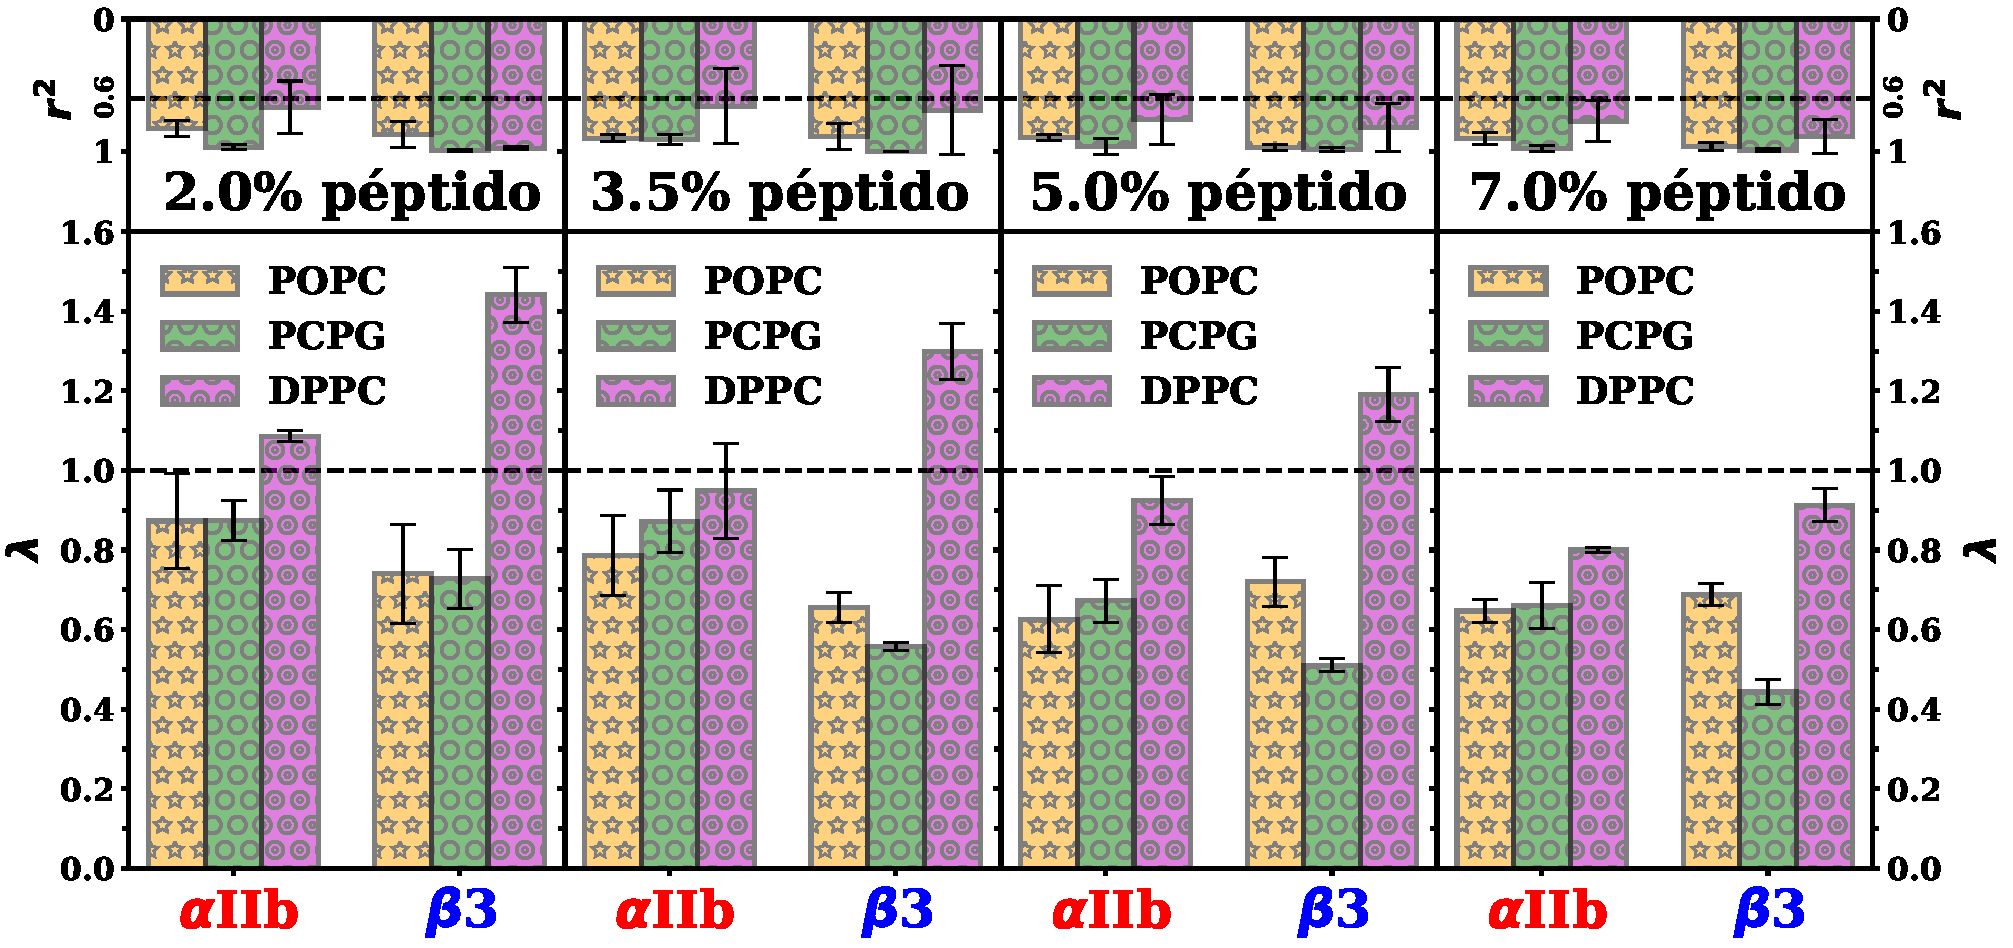
\includegraphics[width=0.99\linewidth]{fig/01_expe/mono/lambda_all2.pdf}
	\caption[Factor $\Lambda$ para las mezclas lípido-péptido.]{Factor $\Lambda$ para las mezclas lípido-péptido. Panel inferior valores de $\lambda$ para cada péptido en diferentes interfases lipídicas y panel superior los respectivos valores de r$^2$.}
        \index{lambda}
    \label{fig:lambda}
\end{figure}
%%%%%%%%%%%%%%%%%%%%% Fin %%%%%%%%%%%%%%%%%%%%%%%%


Se realizó este análisis con las isotermas de las mezclas lípido-péptido el cual se muestra en la \textbf{figura} \ref{fig:lambda}.  Observando los valores de r$^2$ (panel superior) en la mayoria de las mezclas   r$^2$ fue \textgreater{} 0.8, excepto para \ac{dppc} 
(\begin{tikzpicture}
            \node[draw, circle, fill=deepmagenta, line width=0.5pt, inner sep=3pt, scale=0.4, font=\color{black}] {\faCircle};
            \end{tikzpicture}) 
a 2.0\% y 3.5\% donde r$^2$ fue levemente \textgreater{} 0.6. Que r$^2$ se aproxime a 1 indica que las diferencias entre las isotermas reales e ideales están dadas principalmente por el valor de $\lambda$ y son independientes del rango de presión. Respecto al factor $\lambda$, el péptido $\beta$3  tiende a presentar valores de $\lambda$ \textgreater{} 1 en concentraciones de  2.0\% a 5.0\%, mientras que en presencia de $\alpha$IIb, $\lambda$ es ligeramente mayor a 1 cuando la concentración es 2.0\%. Antes se vió que a las dos presiones evaluadas los péptidos inducían una expansión (posiblemente interacciones repulsivas lípido-péptido) sobre la fase de éste lípido lo cual se reafirma con este análisis. Además con el valor agregado que se aprecia a nivel cuantitativo el efecto que induce cada péptido independiente de la presión superficial. Los valores menores de $\lambda$ se obtuvieron en las mezclas PCPG (\begin{tikzpicture}
  \node[draw, circle, fill=black, line width=0.2pt, inner sep=0.05pt, scale=0.6, font=\color{emerald}] {\faCircle}; 
  \end{tikzpicture})-$\beta$3, indicando la presencia de interacciones atractivas lípido-péptido y éstas se intensifican a medida que aumenta la concentración de péptido (disminuye $\lambda$; lo más probable es que el péptido $\beta$3 con carga positiva es atraído por la carga negativa del \ac{popg} en la mezcla PCPG. En cuanto a las mezcla \ac{popc}
  (\begin{tikzpicture}
  \node[draw, circle, fill=black, line width=0.2pt, inner sep=0.5pt, scale=0.4] {};
  \node[star, star point ratio=2.25, draw=black, fill=goldenpoppy, line width=0.2pt, minimum size=0.4cm, inner sep=0pt] {};
\end{tikzpicture})-péptido se obtuvieron valores intermedios respectos a las otras dos interfases, donde tanto $\alpha$IIb como $\beta$3  presentan interacciones atractivas con la interfase neutra.

Para enriquecer y profundizar el análisis de las isotermas de las mezclas lípido-péptido, es pertinente considerar los cambios conformacionales que los lípidos experimentan en respuesta a las distintas acomodaciones del péptido. Este fenómeno puede ser crucial para comprender las interacciones entre los componentes de la mezcla y cómo estas interacciones se modifican en función de la concentración del péptido y la naturaleza de la interfaz lípido-péptido.

Además, el concepto de compactación adquiere relevancia en este contexto. La compactación se refiere a la densificación de la monocapa lipídica inducida por la presencia y la interacción del péptido. Esta densificación puede resultar en un cambio en la movilidad y en la conformación de los lípidos, así como en la interacción entre los lípidos y los péptidos.


\section{Potencial de superficie y momento dipolar en mezclas lípido-péptido}\label{deltaV_mezclas}

Previamente en la \textbf{sección \ref{mono_pept_puros}}  se introdujo el concepto del potencial de superficie y momento dipolar. La \textbf{figura} \ref{fig:mu_dV_alfa} muestra el cambio del $\Delta$V en función del empaquetamiento molecular. Además, se estimó el momento dipolar perpendicular ($\mu_\perp$) empleando la ecuación \ref{ecu:potencial} el cual se muestra en el panel inferior de cada subfigura. Dado que $\Delta$V depende tanto de la densidad de empaquetamiento como de la orientación de las moléculas en la monocapa, se espera un aumento en los valores $\Delta$V durante la compresión de la fase LE como consecuencia de un progresivo  reordenamiento vertical. Este efecto se observó en las monocapas de \ac{dppc} ya que presenta diferentes fases a medida que se comprime, sin embargo, en presencia de péptido sea  \textbf{$\alpha$}IIb o  $\beta$3, disminuyen levemennte el $\Delta$V del lípido puro. La diferencia en valores de $\Delta$V entre las fases LE y LC ($\Delta$V$_{LC}$ -- $\Delta$V$_{LE}$) puede dar cuenta de repulsiones lípido-péptido como ya se mencionó anteriormente. Además se observó cómo la presencia de péptido cambia la forma del potencial del \ac{dppc} puro (señalados con las fechas \textcolor{black}{\faLongArrowRight}). En la interface neutra (\ac{popc}), el cambio del $\Delta$V por la presencia de péptido ($\alpha$IIb ó  $\beta$3) es ligeramente distinguible respecto al lípido puro; y con la interface cargada negativamente (mezcla binaria PCPG) se esperaba ver alguna diferencia notable entre el péptido $\alpha$IIb y $\beta$3 dado que estos tiene carga neta diferente, pero lo observado fue un cambio muy pequeño en presencia de $\beta$3. Esta observación podría atribuirse a la complejidad inherente al control experimental de los rearreglos estructurales y moleculares, así como a la incertidumbre intrínseca en las mediciones realizadas \cite{Brockman1994}. 
El $\mu_\perp$ para \ac{popc} y \ac{dppc} se muestra en la \textbf{figura} \ref{fig:mu_dV_alfa}A-B (panel inferior) en ausencia y presencia de ambos péptidos, cuando el área molecular $\Xapprox 225$  Å\textsuperscript{2}, el $\mu_\perp$ inicia con  valores más altos respecto al $\mu_\perp$  los lípidos puros, y esto se debe a lo ya mencionado, donde a área grandes los péptidos tienen suficiente libertad para tender a orientarse paralelamente a la superficie y por lo tanto, habrán más aminoácidos que entran en contacto con el agua los cuales contribuyen al incremento del $\mu_\perp$. A medida que se comprime lateralmente, los péptidos se reorientan verticalmente, por lo tanto, se observa un decrecimiento paulatino del  $\mu_\perp$ hasta llegar a valores similares que alcanza el lípido puro cuando han colapsado. Con la interfase de PCPG sucedio lo contrario, especialmente en presencia de $\beta$3, donde a áreas mayores el $\mu_\perp$ del lípdio es mayor respecto a las mezcla con $\beta$3. En general para las mezclas lípido-péptido llama la atención en todos casos, siempre se llegó valores similares de la interface puro, al similar fue reportado por Le--Thu Nguyen et al. \cite{Nguyen2010}, donde se observó que el $\mu_\perp$ de diferentes polipéptidos $\alpha$ hélice es significativamente suprimido en soluciones acuosas debido al efecto de la esfera de solvatación de moléculas de agua que pueden formar puentes de hidrógeno con los grupos carbonilos de los péptidos específicamente cuando se encuentran ``paralelo'' a la superficie, luego al comprimirse los $\mu_{H_{2}O}$ se orientan hacia abajo, dando como resultado la diminución del $\mu_\perp$. Además, si consideramos que ambos péptidos tienen resíduos del domino \ac{ic} en la subfase, el $\mu_{péptido}$ de esos residuos ya se encuntran ``apantallados'', por lo tanto, no contribuyen al $\mu_\perp$.


%%%%%%%%%% Potencial y dipolo mezclas %%%%%%%%%%%%

\begin{figure}[H] % supposedly places it here ...
    \centering
	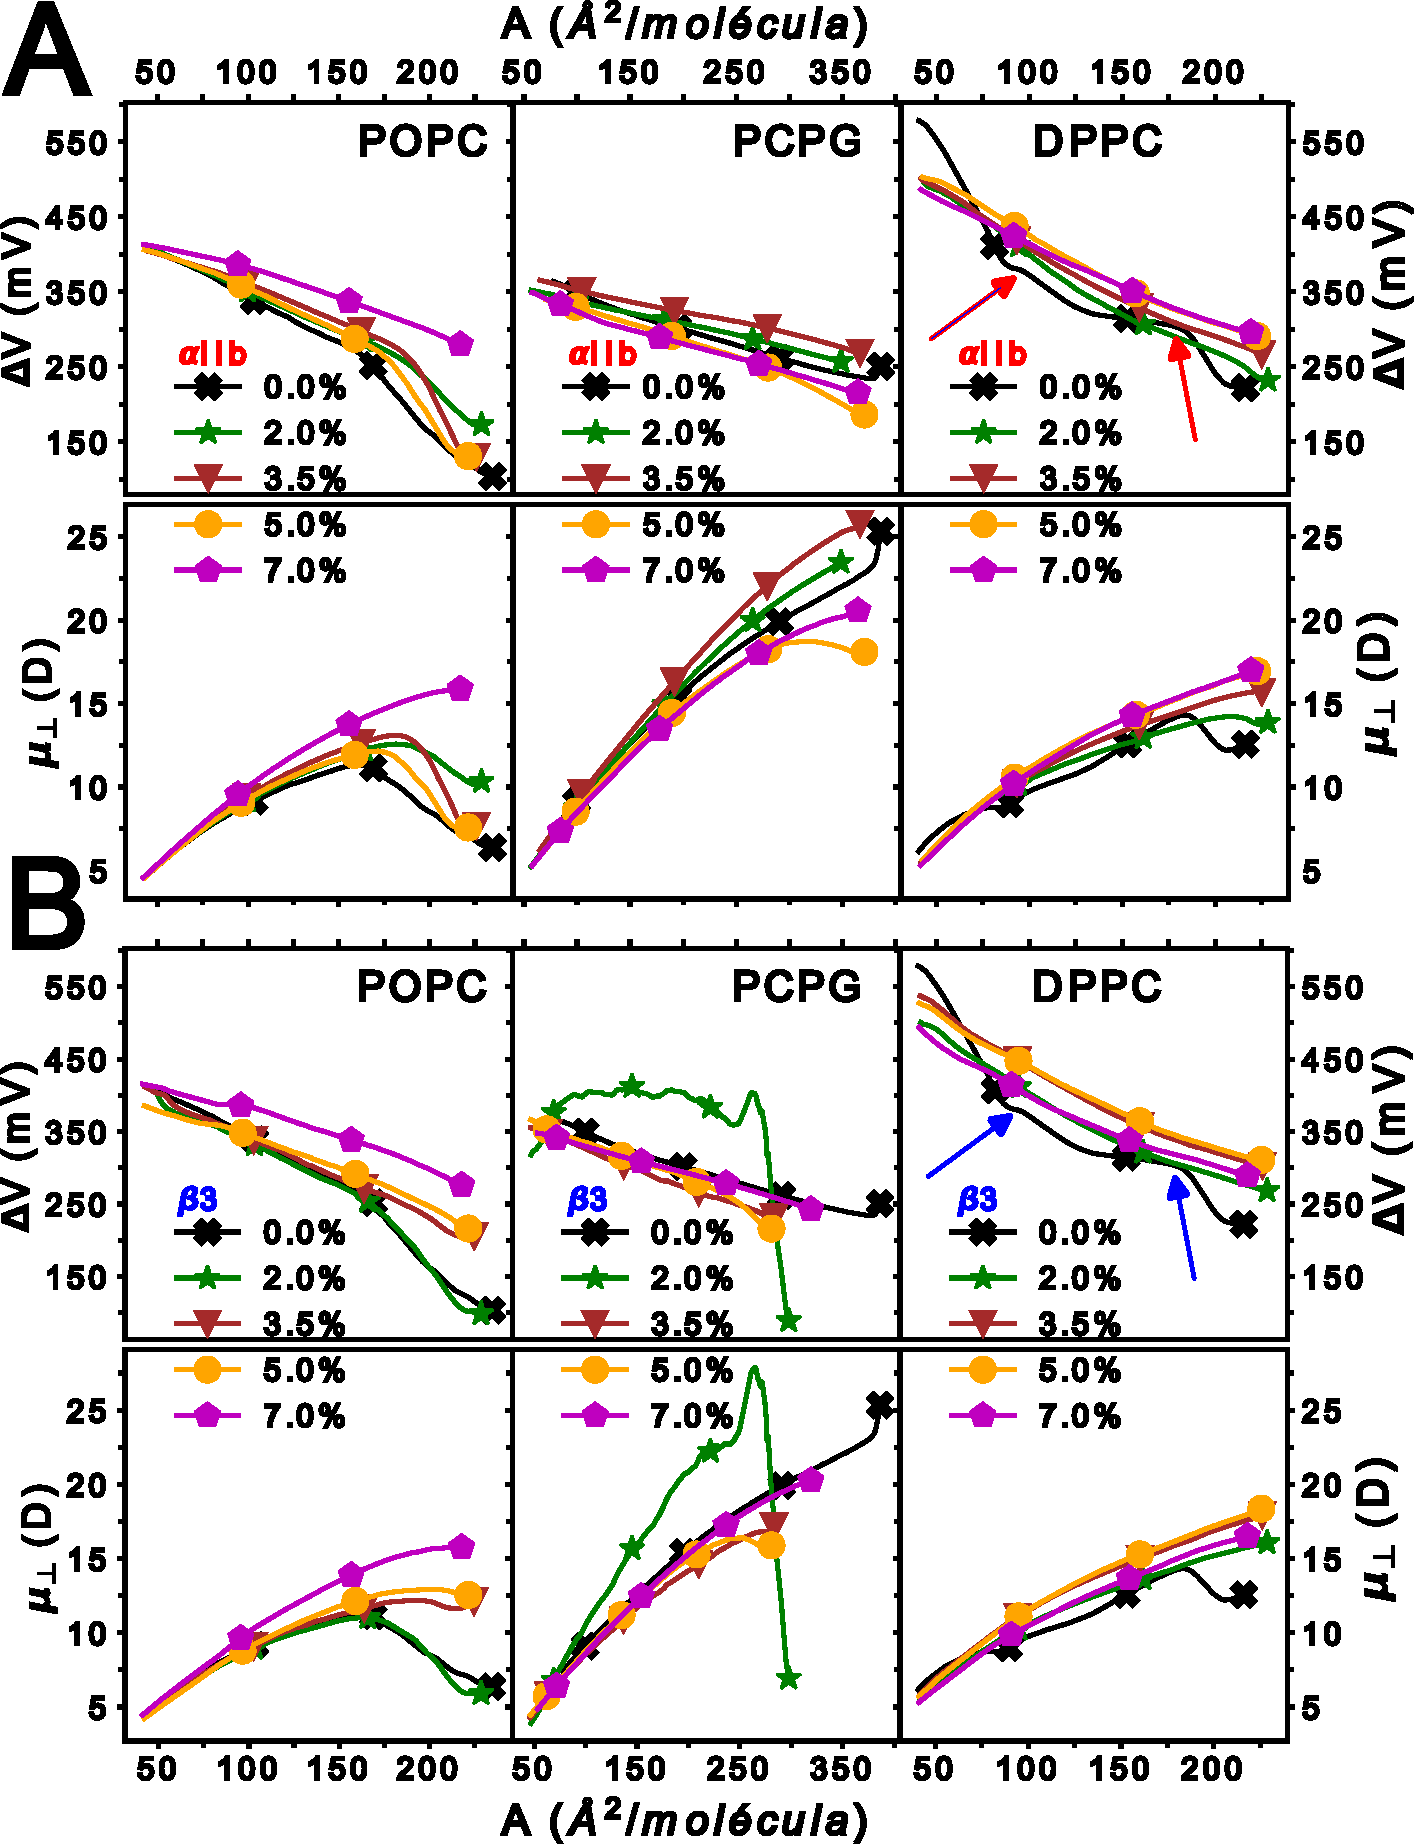
\includegraphics[width=0.99\linewidth]{fig/01_expe/mono/mu_dipolo_deltaV_all.pdf}
	\caption[Potencial de superficie y momento dipolar para las mezclas lípido-péptido]{Potencial de superficie ($\Delta$V)  y momento dipolar perpendicular ($\mu_\perp$) para las mezclas lípido-péptido en función del área molecular promedio (\textbf{A}). A) $\Delta$V (panel superior) y $\mu_\perp$ (panel inferior) para las mezclas lípido/$\alpha$IIb. B) $\Delta$V (panel superior) y $\mu_\perp$ (panel inferior) para las mezclas lípido/$\beta$3.}
        \index{mu_dV_alfa}
    \label{fig:mu_dV_alfa}
\end{figure}
%%%%%%%%%%%%%%%%%%%%% Fin %%%%%%%%%%%%%%%%%%%%%%%%



\section{Análisis de la elasticidad lateral}
%%https://www.cell.com/biophysj/pdf/S0006-3495(97)78226-2.pdf
%%%Leer bien para posible análisis extra del módulo
%%%https://hal.science/hal-04037820/document

La membrana celular es una organización compleja y muy dinámica. Su integridad y funcionalidad dependen de la flexibilidad estructural de sus componentes. La mutua influencia entre componentes, principalmente lípidos y proteínas, puede modular la deformación, los cambios en radios y curvatura, cambios en el espesor de la membrana. Particularmente, la compresibilidad lateral de la membrana es un parámetro que describe sus propiedades mecánicas y puede ser controlada por la composición de la membrana y/o por la presencia de proteínas que inducen estos cambios \cite{Evans1976}. Para examinar la rigidez lateral de las monocapas, específicamente en las mezclas lípido-péptido, se calculó el módulo de compresibilidad (C$_s^{\text{--}1}$) usando los datos de las curvas $\pi \text{--}$\textit{A} (\textbf{figura} \ref{fig:area_pi_all})  basado en la ecuación \ref{ecu:Cs}, 

\begin{equation}\label{ecu:Cs}
    C_s^{\text{--}1} =  \text{--} A \left(\frac{d\pi}{dA} \right)  
\end{equation}

Donde \textit{A} es el área por molécula a la presión superficial  $\pi$. El C$_s^{\text{--}1}$ provee información acerca de la conformación estructurada de los lípidos y la rigidez de la monocapal. Lípidos con una conformación estructurada (fase LC), presentarán valores de C$_s^{\text{--}1}$ altos, mientras que si presentan un cierto grado de heterogeneidad estructural (fase LE), C$_s^{\text{--}1}$ tendrá valores bajos. Valores cercanos a cero de C$_s^{\text{--}1}$, corresponden una interfase de agua pura, libre de monocapas. Si hay un incremento en su magnitud estará dada por la actividad superfical de las moléculas presentes en la interface, cuando el valor C$_s^{\text{--}1}$ es grande, significa que la monocapa es menos compresible. Valores de C$_s^{\text{--}1}$ cercanos a cero corresponden a una interfase de agua pura, libre de monocapa. La fase \ac{le} se caracteriza por presentar una C$_s^{\text{--}1}$ entre 12-50 mN/m, y valores entre 100-250 mN/m corresponde a una fase LC \cite{Hadjittofis2017}. La \textbf{figura} ~\ref{fig:CsPi} muestra los curvas de compresibilidad tanto para los componentes puros como las mezlcas lípido-péptido, lípido-$\alpha$IIb se observan al lado derecho y al lado izquierdo lípido-$\beta$3.
%%2019_Agata_Ladniak.pdf 
Respecto a los péptidos puros, ambos alcanzan rápidamente C$_s^{\text{--}1}$ $\Xapprox$  30 mN/m y permanece oscilando en ese valor hasta presiones altas. Además, los dos péptidos presentan un pequeño decrecimiento de C$_s^{\text{--}1}$ alrededor de los 28 mN/m y 32 mN/m para $\alpha$IIb y $\beta$3, respectivamente. Este mínimo podría atribuirse a una reorganización estructural de los péptidos en la interfase tal como se mencionó en las \textbf{secciones \ref{sect:mono_mezclas}} y \textbf{\ref{deltaV_mezclas}} \hl{(buscar refencias de Cs para péptidos mostrar con flecha en la gráfica el minimo de los péptidos y del dppc)}.
Observando los C$_s^{\text{--}1}$ para \ac{popc} puro, éste alcanza valores máximos hasta $\Xapprox$ 50 mN/m (valores característicos para una fase LE) y una vez alcanza la presión de colapso decae. En general en presencia de péptido $\alpha$IIb  o $\beta$3 el C$_s^{\text{--}1}$ disminuye respecto al lípido puro y éste efecto es más marcado con $\beta$3. 
Con la interfase que tiene un 30\% mol de \ac{popg}, éste disminuyó C$_s^{\text{--}1}$ del \ac{popc} puro, donde esta mezcla PCPG presentó un C$_s^{\text{--}1}$ de  $\Xapprox$ 30 mN/m, valor muy similar al de los péptidos (\textbf{figura} ~\ref{fig:CsPi} panel del medio). En prencia de péptido, éstos tienden a disminuir la compresibilidad del PCPG puro sutilmente, siendo $\alpha$IIb  el péptido que induce un mayor efecto.
Finalmente en la interfase con \ac{dppc}, para el lípido puro se observan dos estados, el primero alcanza un valor de C$_s^{\text{--}1}$  $\Xapprox$ 25 mN/m, éste primer estado corresponde a la coexistencia de fase LE--LC \hl{buscar REF}. Posteriormente se produce un aumento pronunciado del C$_s^{\text{--}1}$ con el amento de la $\pi$ hasta alcanzar valores de C$_s^{\text{--}1}$  mayores a 100 mN/m, el cual se atribuye un estado de fase LC. Cuando se adiciona péptido ya sea $\alpha$IIb o $\beta$3, ambos disminuyen la compresibilidad del lípido drasticamente, incluso a bajas comcentraciones del 2.0\% de péptido pasa a tomar valores cercanos a $\Xapprox$ 50 mN/m, donde $\beta$3 es el más disminuye C$_s^{\text{--}1}$.

Para finalizar en la \textbf{tabla} \ref{tab:resum_mono} se muestras un resumen de las propiedades de todas las monocapas estudiades en éste trabajo, se tomó como referencia una presión de 30 mN/m.

%%%%%%%%%%%%%%%%%%%Tabla resumen%%%%%%%%%%%%%%%%%%%%%%%%
% Please add the following required packages to your document preamble:
% \usepackage{booktabs}
% \usepackage{multirow}
\begin{table}[H]
\centering
%\begin{adjustbox}{width=1\textwidth}
\caption{Resumen propiedades  monocapas a una presión de 30 mN/m.\hl{Falta completar} }\label{tab:resum_mono}
\resizebox{\textwidth}{!}{
\begin{tabular}{@{}cclllllllllll@{}}

\toprule
\multirow{2}{*}{Péptido} & \multirow{2}{*}{\%}  & \multicolumn{3}{c}{$\mu_\perp$ (D)}  & \multicolumn{1}{p{0.01mm}}{}  & \multicolumn{3}{c}{C$_s^{\text{--}1}$ (mN/m)} & \multicolumn{1}{p{0.01mm}}{}  & \multicolumn{3}{c}{A (Å\textsuperscript{2})} \\ 

\cmidrule(lr){3-5} \cmidrule(lr){7-9} \cmidrule(l){11-13}  
                         &                      & \multicolumn{1}{c}{POPC} & \multicolumn{1}{c}{PCPG} & \multicolumn{1}{c}{DPPC} & \multicolumn{1}{p{0.01mm}}{} & \multicolumn{1}{c}{POPC} & \multicolumn{1}{c}{PCPG} & \multicolumn{1}{c}{DPPC} & \multicolumn{1}{p{0.01mm}}{} & \multicolumn{1}{c}{POPC} & \multicolumn{1}{c}{PCPG} & \multicolumn{1}{c}{DPPC} \\ 
                         
                                                
\cmidrule(lr){1-2} \cmidrule(lr){3-5} \cmidrule(lr){7-9} \cmidrule(l){11-13}

- - -     		& 0.0					& ab\textpm 0.01		& ab\textpm 0.00		& ab\textpm 0.00		& 	&54.96\textpm b		& 36.39\textpm b		& 130.80\textpm b& &	73.69\textpm 3.70 & 100.51\textpm 4.35 &  39.06\textpm 0.55 
\vspace{3mm} \\

$\alpha$IIb     & \multirow{2}{*}{2.0}   &  6.64\textpm 0.01 	& 9.86\textpm 0.00	& 9.71\textpm 0.00	& 	& 44.92\textpm b		& 30.13\textpm b		& 63.23\textpm b	& & 65.30\textpm 2.31 	& 75.32\textpm 2.63& 58.36\textpm 0.06\\ 
$\beta$3        & 						&  7.50\textpm 0.00 	& 12.03\textpm 0.12	& 10.03\textpm 0.01	& 	& 47.12\textpm b		& 34.28\textpm b		& 46.28\textpm b	& &	61.98\textpm 2.42 	& 72.45\textpm 5.64& 63.80\textpm 0.07                          
\vspace{3mm}\\

$\alpha$IIb     & \multirow{2}{*}{3.5} 	&  8.70\textpm 0.00	& 10.56\textpm 0.07	& 10.21\textpm 0.00	& 	& 45.45\textpm b		& 27.30\textpm b		& 52.51\textpm b	& &	74.24\textpm 0.55	& 90.15\textpm 24.02& 60.94\textpm 0.81\\
$\beta$3        & 						&  7.40\textpm 0.00	& 8.19\textpm 0.07	& 11.88\textpm 0.00	& 	&53.41\textpm b		& 38.27\textpm b		& 41.73\textpm b	& &	65.02\textpm 1.43 	&65.04\textpm 0.67& 69.83\textpm 7.57                           
\vspace{3mm} \\

$\alpha$IIb     & \multirow{2}{*}{5.0}   &  8.68\textpm 0.00	& 8.71\textpm 0.03	& 11.36\textpm 0.00	& 	&49.57\textpm b		& 31.39\textpm b		& 51.91\textpm b	& &	71.41\textpm 6.89 	&77.62\textpm 5.07& 65.76\textpm 1.74\\
$\beta$3        & 						&  7.61\textpm 0.00	& 7.31\textpm 0.00	& 12.77\textpm 0.01	& 	&33.06\textpm b		& 32.27\textpm b		& 44.45\textpm b	& &	74.34\textpm 3.09 	& 59.47\textpm 1.06& 71.83\textpm 1.51                          
\vspace{3mm} \\

$\alpha$IIb    & \multirow{2}{*}{7.0}  	&  9.89\textpm 0.00	& 10.53\textpm 0.00	& 11.51\textpm 0.00	& 	&45.63\textpm b		& 32.72\textpm b		& 47.61\textpm b	& &	81.54\textpm 0.89 	&85.71\textpm 4.51& 64.21\textpm 0.41\\
$\beta$3       & 						&  9.06\textpm 0.00	& 9.33\textpm 0.31	& 10.24\textpm 0.00	& 	&31.09\textpm b		& 31.85\textpm b		& 43.02\textpm b	& &	76.34\textpm 1.32 	& 59.57\textpm 13.07& 68.88\textpm 1.94  \\ 
\bottomrule
\end{tabular}
}
\end{table}                        
%%%Fin Tabla resumen%%%


%%%%%%%%%% Figura Módulo de compresibilidad %%%%%%%%%%%%

\begin{figure}[H] % supposedly places it here ...
    \centering
	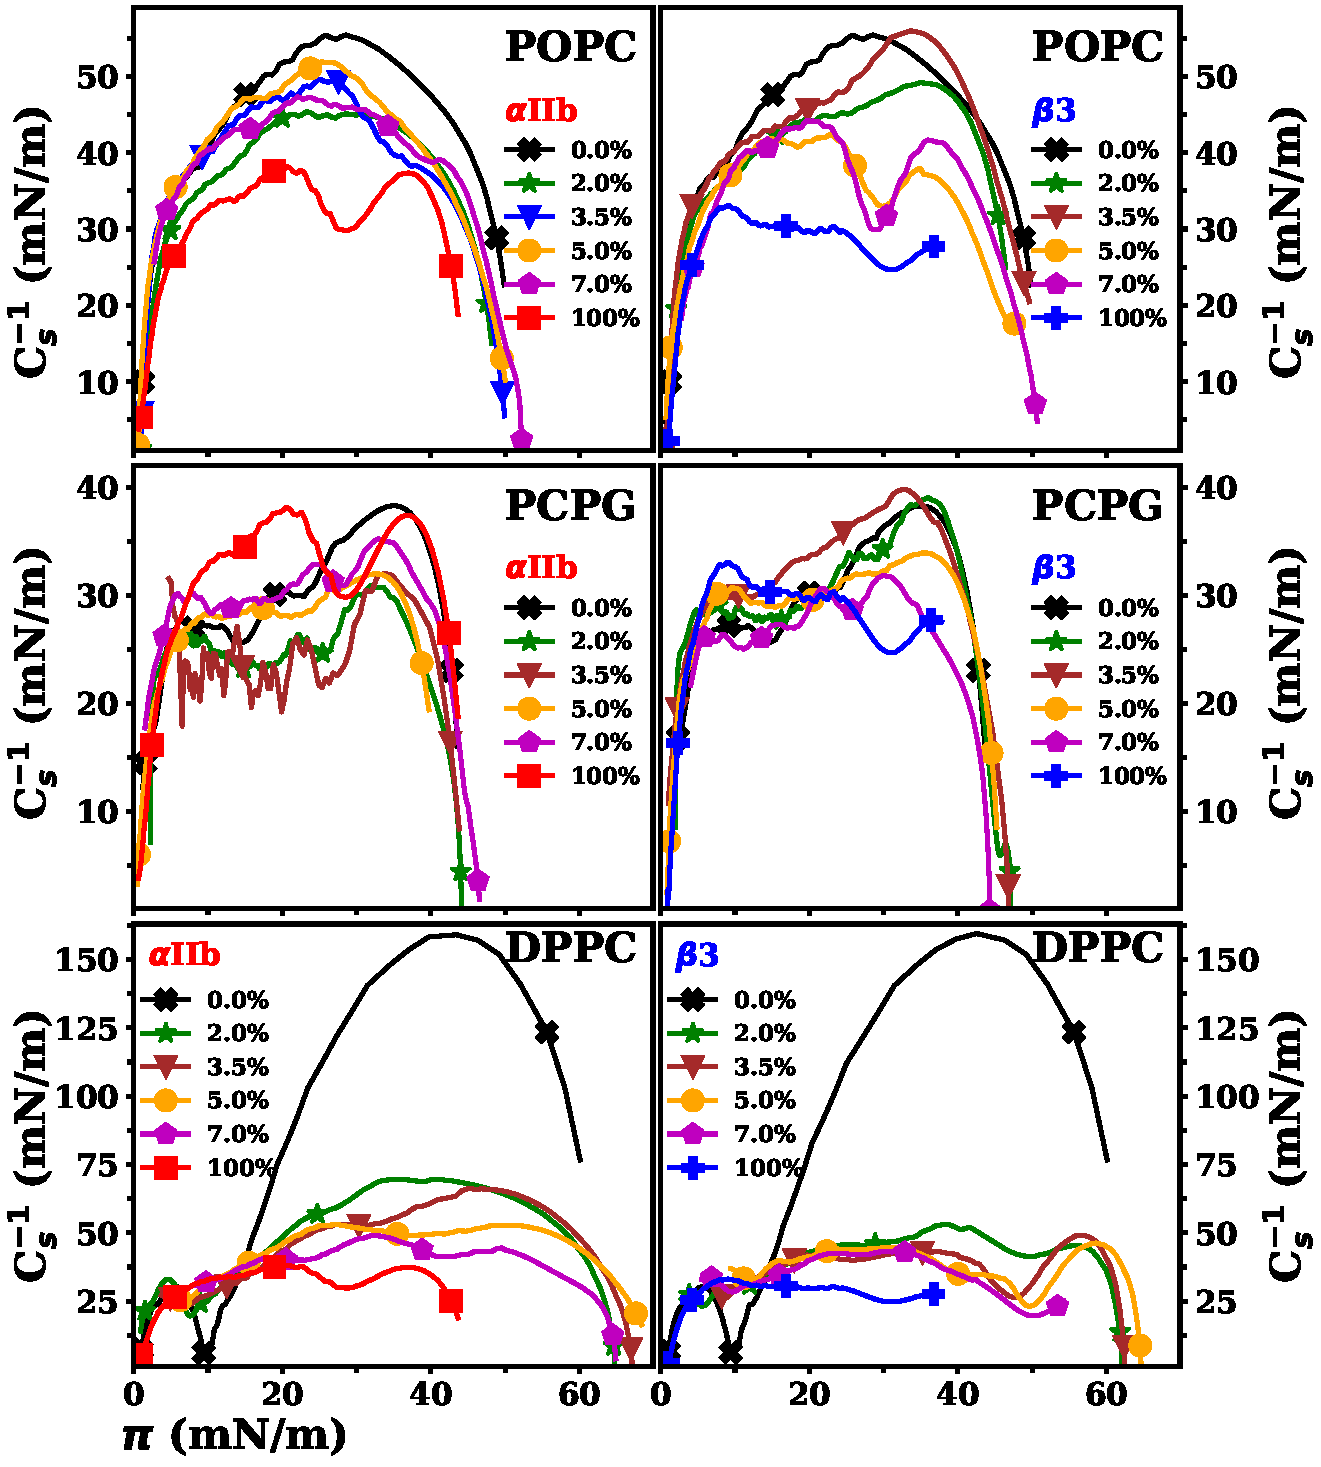
\includegraphics[width=0.99\linewidth]{fig/01_expe/mono/cs_all.pdf}
	\caption[Módulo de compresibilidad  en fucnión de la presión superficial en la interfase aire-agua.]{Módulo de compresibilidad (C$_s^{\text{--}1}$ ) en función de la presión superficial ($\pi$) en la interfase aire-agua. Al lado izquierdo lípido/$\alpha$IIb y lado derecho lípido/$\beta$3.}
        \index{CsPi}
    \label{fig:CsPi}
\end{figure}
%%%%%%%%%%%%%%%%%%%%% Fin %%%%%%%%%%%%%%%%%%%%%%%%


%%%%%%%%% Ciclos compresion-Expansión%%%%%%
\section{Discusión general del capítulo}

Para resumir de forma gráfica los resultados observados anteriormente, la \textbf{figura} \ref{fig:esquema_final} ilustra lo planteado en cada sistema. Se mencionó que la orientación de los péptidos puros en monocapas de Langmuir es perpendicular al plano de las monocapas, preferentemente. Donde al inicio a presiones bajas éstos presentan una conformación acostada sobre la fase acuosa pero a medida que se comprime lateralmente, éstos se orientan verticalemente. Además, dicha orientación es en dirección del N al C terminal debido a que los dos péptidos tienen resíduos polar en la región del C terminal que pueden interactuar favorablemente con el agua, mientras que la región del N terminal tiene un carácter más hidróbico que podría presentar interacciones poco favorables con el agua. También se mencionó que esta región del C terminal que está en contacto con la interfase, posiblemente presenta rearreglos de estructura secundaria de tal forma que a medida que se comprime, esta región adopta una estructura helicoidal donde algunos residuos polares contribuyen al potenecial de superficie. Respecto al efecto que inducen los péptidos $\alpha$IIb/$\beta$3 sobre monocapas de lípidos, en la caso de la interfase neutra y de características de \ac{le}, ambos péptidos inducen un efecto de compactación, es decir, hay presecia de interacciones lípido-péptido atractivas que llevan la monocapa a un estado más compacto respecto a la monocapa del lípido puro. Si a la misma interfase se le agrega un 30\% de lípido con carga negativa como es el \ac{popg}, los péptidos inducen un efecto opuesto, mencionado anteriormente, es decir, se observó una interacción repulsiva, siendo esta mayor en presencia de $\beta$3. Por otra parte, cuando los péptidos estan en una interfase lípidica neutra pero con cadenas saturadas como el \ac{dppc}, estos inducen un efecto repulsivo sobre la monocapa de los lípidos, incluso para ésta interfase se vio que ya con un 2\% de péptido disminuye drásticamente la compresiblidad respecto al lípido puro, miestras que las compresibilidades de las interfaces \ac{popc} y PCPG también dismuyen pero el efecto es menos marcado que con \ac{dppc}.

\begin{figure}[h] % supposedly places it here ...
    \centering
	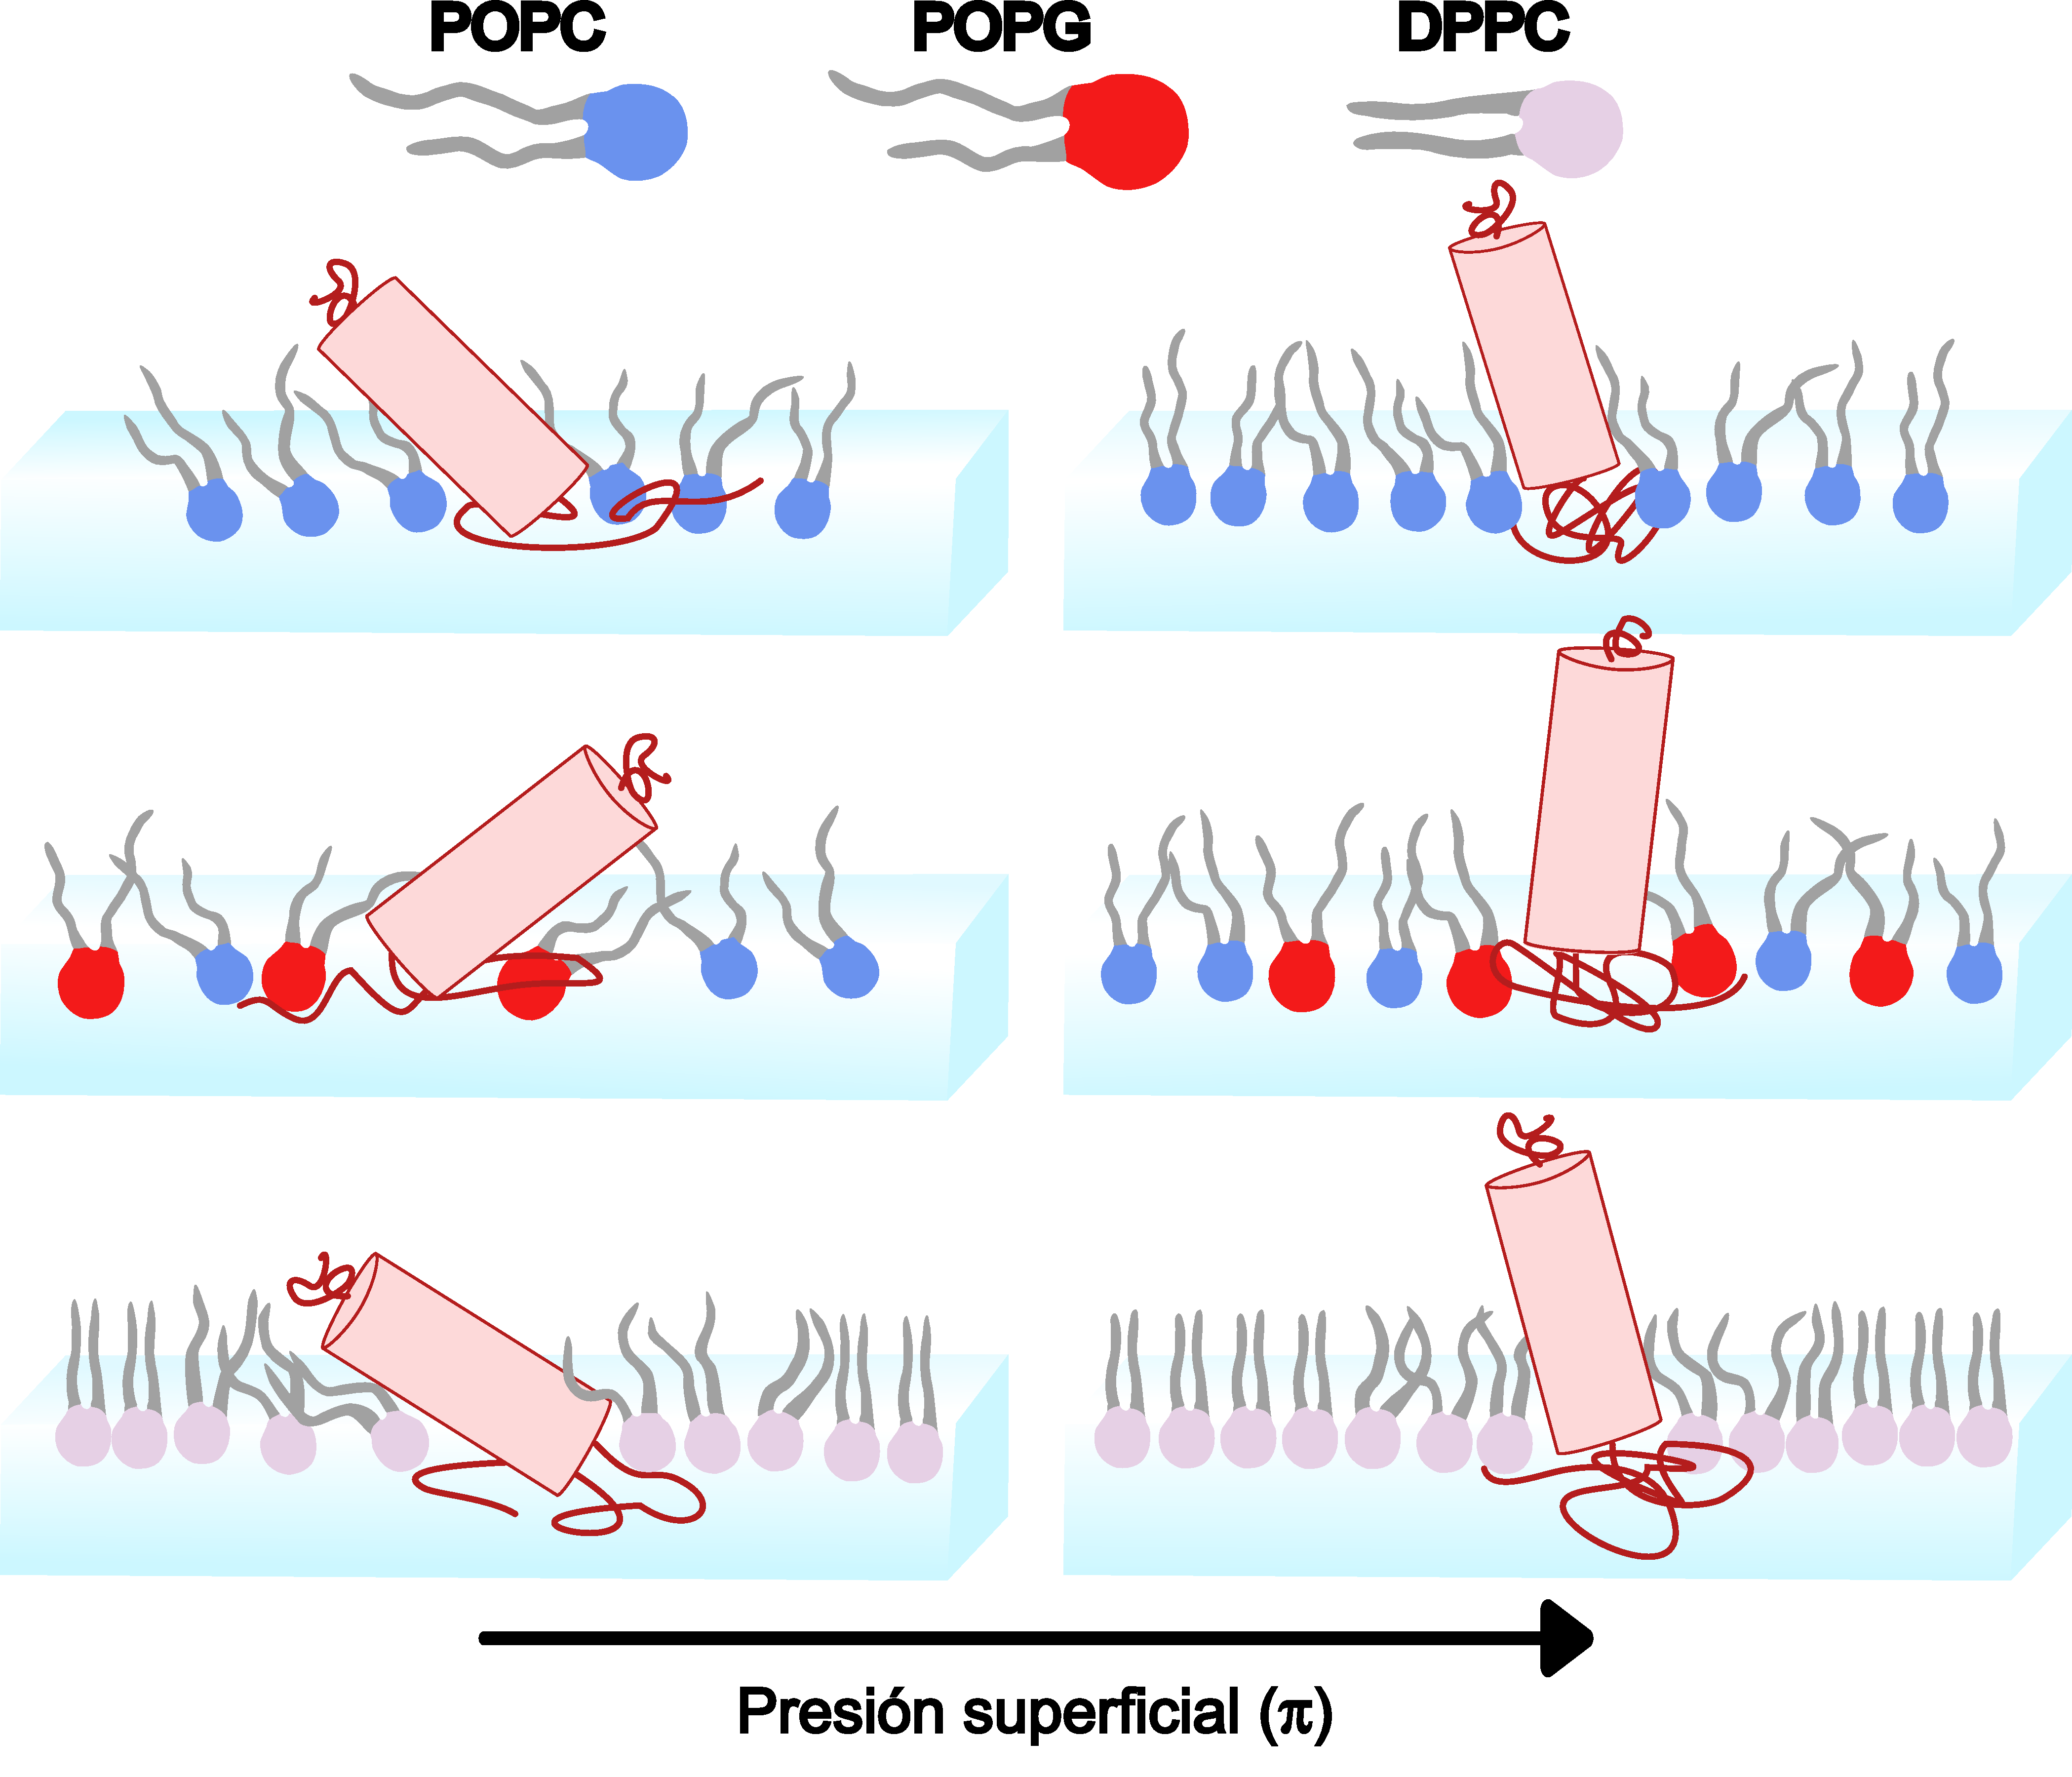
\includegraphics[width=0.99\linewidth]{fig/01_expe/esquema_final_lipido-peptido.pdf}
	\caption[Esquema de interacción lípido-péptido en monopas]{Esquema de interacción lípido-péptido en monopas. A la izquierda representación en condiciones iniciales de presión superficial cercano a cero; a la derecha, reorganización molecular a presiones altas.}
        \index{test}
    \label{fig:esquema_final}
\end{figure}
%%%%%%%%%%%%%%%%%%%%%% Fin %%%%%%%%%%%%%%%%%%%%%%%%
%